\documentclass[a4paper,14pt]{extarticle}

\usepackage[utf8]{inputenc}
\usepackage[T2A]{fontenc}
\usepackage[english, russian]{babel}
\usepackage{amsmath}
\usepackage{amsfonts}
\usepackage{mathtools}
\usepackage{datetime}
\usepackage[pdftex]{graphicx}
\usepackage{indentfirst}
\usepackage{asymptote}
\usepackage{systeme}
\usepackage{listings}
\usepackage[usenames,dvipsnames]{color}	
\usepackage[font={small,it}]{caption}
\newcommand{\Span}{\text{Span}}
\newcommand{\Img}{\text{Im}}
\newcommand{\Ker}{\text{Ker}}


\begin{document}
	\begin{titlepage}
		
		\setlength{\parindent}{0ex}
		
		\begin{center}
			\textsc{
				\vspace{1ex}
				Научно исследовательский университет ИТМО \\
				\vspace{0.5ex}
				Факультет систем управления и робототехники \\
				\vspace{0.5ex}
			}
		\end{center}
		
		\vspace{50mm}
		
		\begin{center}
			Отчет по лабораторной работе №4 \\
			Динамические системы
		\end{center}
		
		\vspace{50mm}
		
		\begin{minipage}{.55\linewidth}
			Выполнил студент группы R3280
			
			\smallskip
			
			Преподаватель
		\end{minipage}
		\hfill
		\begin{minipage}{.4\linewidth}
			\begin{flushright}
				Мовчан И. Е.
				\\
				Перегудин А. А.
			\end{flushright}
		\end{minipage}
		
		\vfill
		\begin{center}
			Санкт-Петербург
			\\
			2024
		\end{center}
		
	\end{titlepage}

	В лабораторной работе имеем дело с непрерывными ($t \in \mathbb{R}$) и дискретными ($k \in \mathbb{Z}$) линейными динамическими системами второго порядка вида
	\[
	\systeme{\dot{x} _1(t) = a_1 x_1(t) + a_2 x_2 (t), \dot{x} _2(t) = a_3 x_1 (t) + a_4 x_2 (t)}
	\quad \quad
	\systeme{x _1(k+1) = a_1x_1(k) + a_2x_2(k), x _2(k+1) = a_3 x_1(k) + a_4 x_2(k)}
	\]
	или в виде одного уравнения:
	\[
	\dot{x}(t) = Ax(t), \quad \quad x(k+1) = Ax(k),
	\]
	где $A \in \mathbb{R}^{2\times2}$
	\section{Изучаем и визуализируем непрерывное}
	Зададим вектора 
	$v_1 = 
	\begin{bmatrix}
		1 \\
		1
	\end{bmatrix}, \
	v_2 =
	\begin{bmatrix}
		-3 \\
		5
	\end{bmatrix} \in \mathbb{R}^2$.
	Ясно, что за устойчивость, собственные вектора и числа отвечает матрица $A$ системы, так как общее решение при том учёте, что A диагонализуема, имеет вид
	\[
	x(t) = e^{\lambda_1t}u_1 + e^{\lambda_2t}u_2,
	\]
	где $u_i$ - собственные вектора матрицы. Случай же с матрицей, не имеющей спектрального разложение, схож (там лишь нужно перейти от треугольной матрицы в базисе из собственных и присоединенных векторов в исходный базис и изучать решение системы с полученной матрицей $B$), поэтому в дальнейшем практически всё время будем исследовать именно матрицы систем, обладающих следующими свойствами:
	\subsection{Асимптотическая устойчивость}
	Зададим матрицу
	\[A = 
	\begin{bmatrix}
		-5 & \phantom{-}3 \\
		\phantom{-}5  & -7
	\end{bmatrix}
	\]
	
	Она имеет собственные числа $\lambda_1 = -2,\ \lambda_2 = -10$ и отвечающие им собственные вектора $v_1$ и $v_2$, приведенные выше.
	
	Решение тогда запишется в следующем виде 
	\[
	x(t) = 
	\alpha e^{-10t} v_1 + \beta e^{-2t} v_2
	=
	 \alpha e^{-10t}
	\begin{bmatrix}
		1 \\ 1
	\end{bmatrix}
	+ \beta e^{-2t}
	\begin{bmatrix}
		-3 \\ 5
	\end{bmatrix}
	,
	\]
	где $\alpha \text{ и } \beta$ зависят от начальных значений, то есть от $x_0 = x(0)$.
	Очевидно, что экспонента в отрицательной степени на бесконечности заглушит любой начальный вектор, поэтому система является асимптотически устойчивой по определению. Изучим теперь ситуацию, в которой $x(0) = \alpha v_1$, $\alpha \in \mathbb{R}$ - произвольное вещественное число. Решение примет вид
	\[
	x(t) = \alpha e^{-10t}
	\begin{bmatrix}
		1 \\ 1
	\end{bmatrix},
	\]
	откуда видим, что $x(t) \in \Span \{v_1\}$. Проводя аналогичные рассуждения для ситуации $x(0) = \beta v_2$ имеем $x(t) \in \Span \{v_2\}$. Наглядно убедимся в полученных результатах:
	
	\begin{figure}[h]
		\centering
		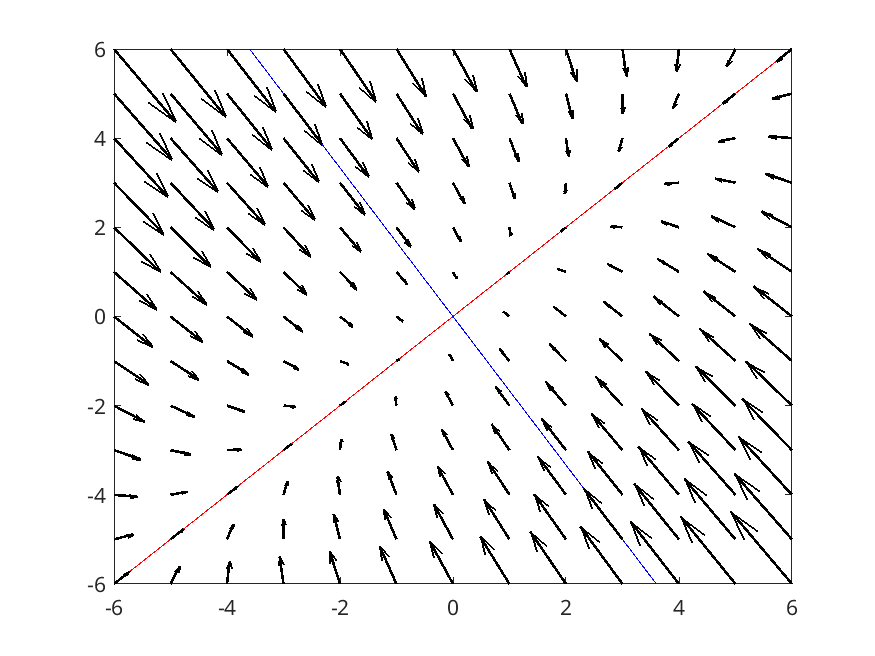
\includegraphics[scale=0.75]{./images/1.png}
		\caption{Фазовый портрет системы}
	\end{figure}	
	
	Видим, что направление всех кривых направлено в $(0, 0)$, то есть система является асимптотически устойчивой. Рядом с прямыми наблюдаем завихрения, говорящие о том, что эти самые прямые являются по сути линейной оболочкой собственных векторов $v_1$ и $v_2$. Также можем различить кривые, которые двигаются строго по этим прямым, что подтверждает верность рассуждений про начальные вектора системы.
	
	Зададим теперь различные начальные значения и выведем графики интегральных кривых, а также зависимости $x_2(x_1)$ для каждых начальных условий:
	
	\begin{figure}[h]
		\centering
		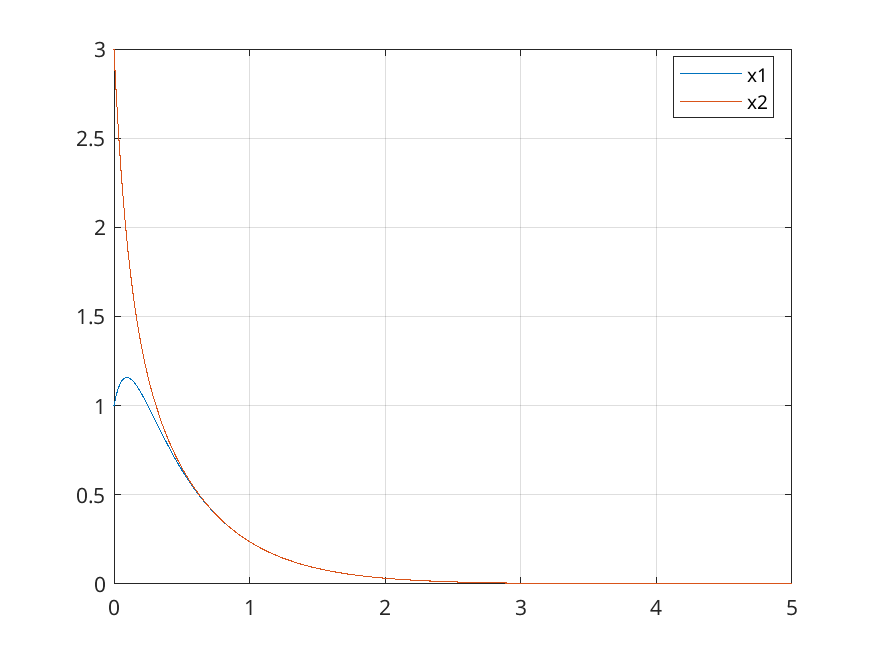
\includegraphics[scale=0.75]{./images/1_1.png}
		\caption{Графики для начальных условий $(1, 3)$}
	\end{figure}
	
	\begin{figure}
		\centering
		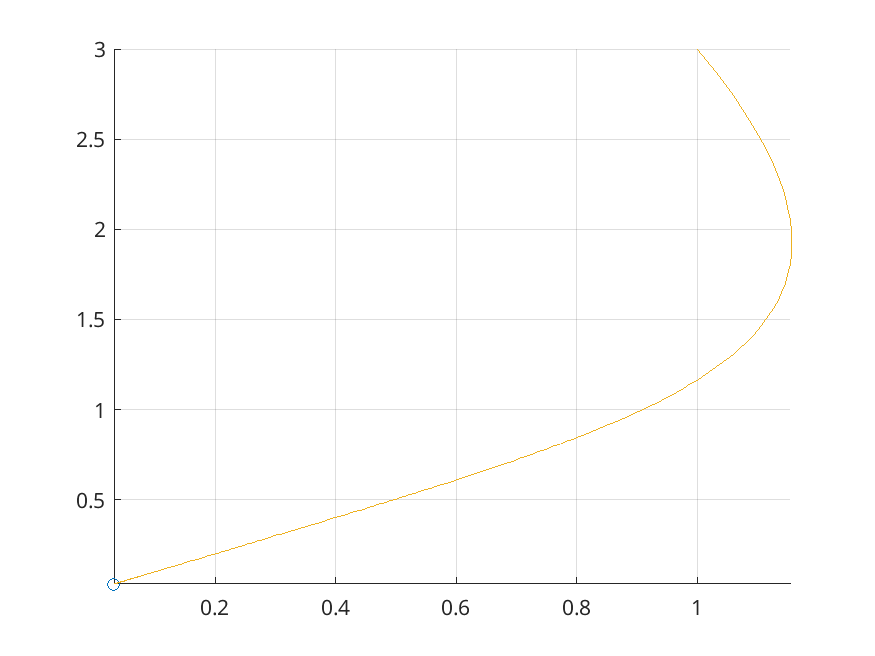
\includegraphics[scale=0.75]{./images/1_comet_1.png}
		\caption{График зависимости $x_2(x_1)$}
	\end{figure}
	
	\begin{figure}
		\centering
		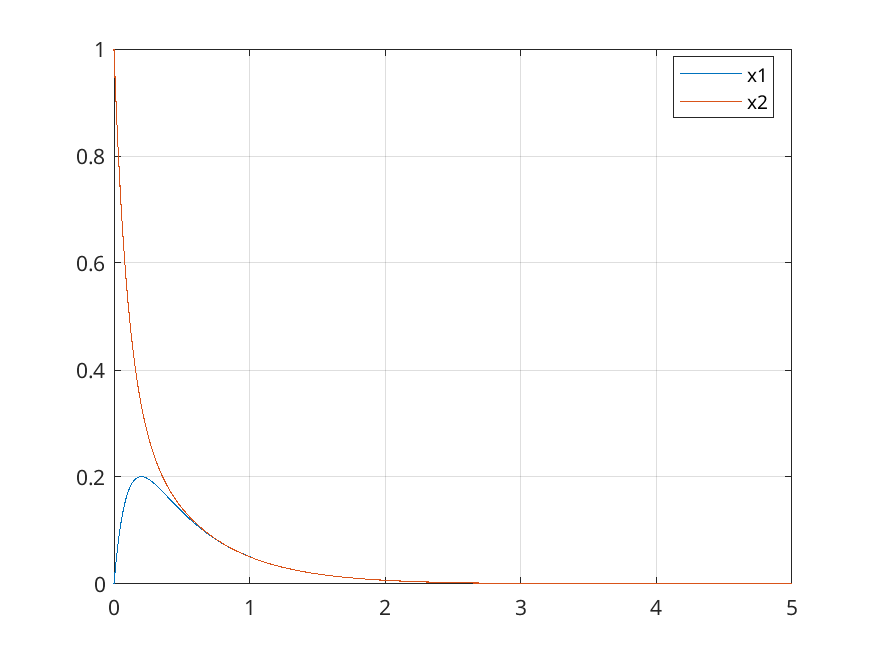
\includegraphics[scale=0.75]{./images/1_2.png}
		\caption{Графики для начальных условий $(0, 1)$}
	\end{figure}
	
	\begin{figure}
		\centering
		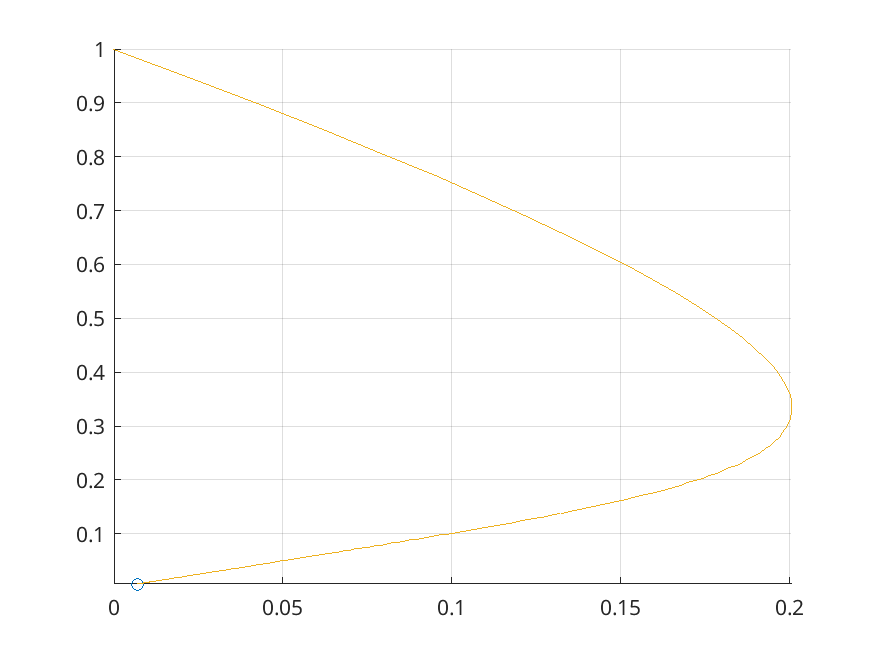
\includegraphics[scale=0.75]{./images/1_comet_2.png}
		\caption{График зависимости $x_2(x_1)$}
	\end{figure}
	
	\begin{figure}
		\centering
		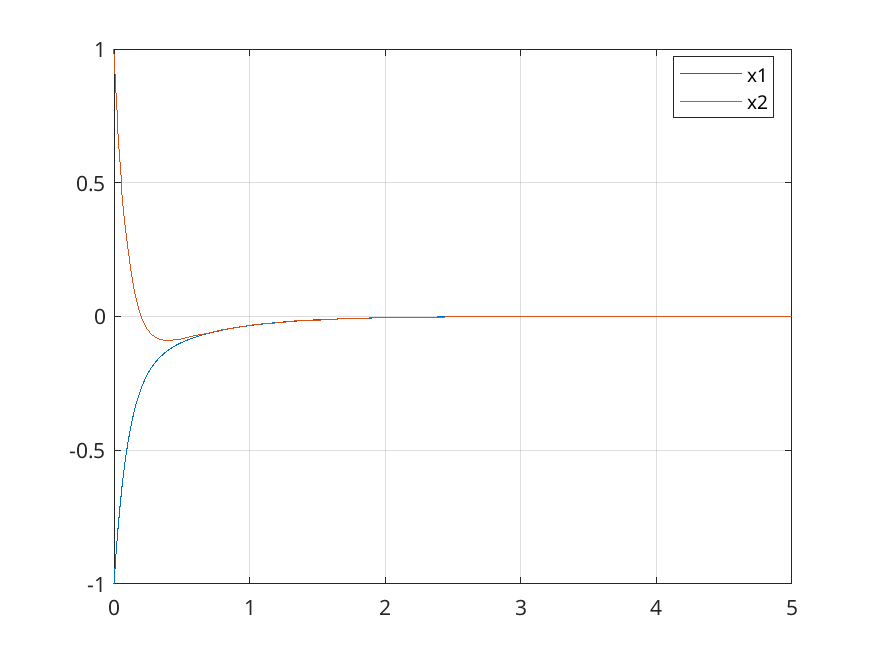
\includegraphics[scale=0.75]{./images/1_3.png}
		\caption{Графики для начальных условий $(-1, 1)$}
	\end{figure}
	
	\begin{figure}
		\centering
		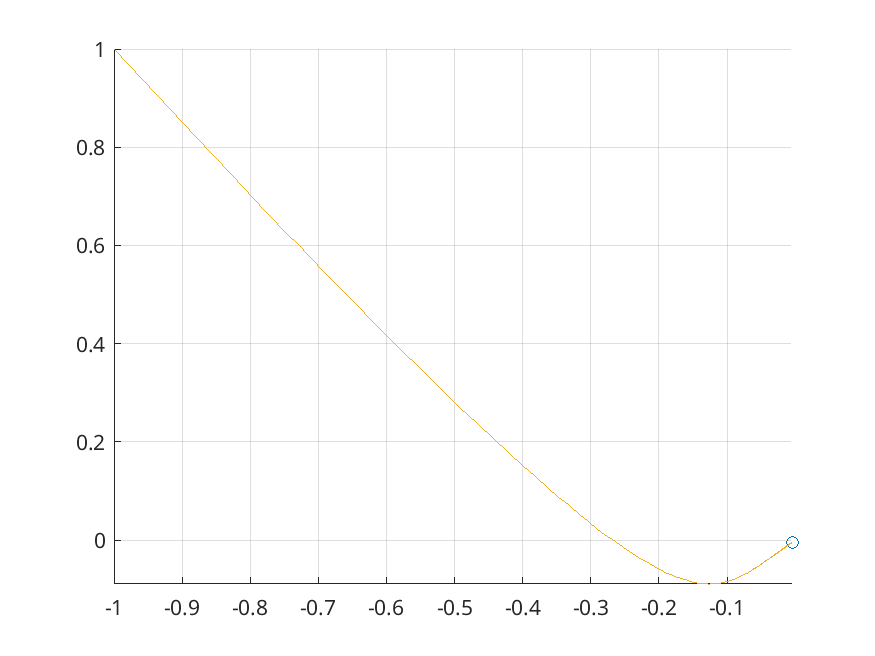
\includegraphics[scale=0.75]{./images/1_comet_3.png}
		\caption{График зависимости $x_2(x_1)$}
	\end{figure}	
	
	\pagebreak
	
	\subsection{Неустойчивость и один собственный вектор}
	Отсутствие двух неколлинеарных собственных векторов и неустойчивость системы нам может дать матрица $A$ с одним положительным собственным числом, алгебраической кратности 2, геометрической - 1. Такой, например, является матрица
	\[A =
	\begin{bmatrix}
		3 & -1 \\
		1 & \phantom{-}1
	\end{bmatrix}.
	\]
	Нетрудно убедиться, что характеристическое уравнение имеет вид 
	\[
	(3-\lambda)(1-\lambda) + 1 = 3 - 4\lambda + \lambda^2 + 1 = \lambda^2 - 4\lambda + 4 = (\lambda - 2)^2 = 0 \Rightarrow \lambda_{1, 2}=2
	\]
	\[A - \lambda E =
	\begin{bmatrix}
		1 & -1 \\ 
		1 & -1
	\end{bmatrix} \Rightarrow v_1 = 
	\begin{bmatrix}
	1 \\ 1
	\end{bmatrix}
	\]
	
	Держа в голове общее решение систем дифференциальных уравнений, получаем неустойчивую систему (в силу $\lambda>0$, то есть бесконечно растующей экспоненты) с одним собственным вектором, чего и хотелось добиться.
	
	Договоримся также, что далее так подробно решения расписывать не будем (потому что умереть можно, если каждый раз писать про одно и то же с разными значениями). Будет приводиться матрица с краткими пояснениями по структуре в случае необходимости, а также её собственные вектора, значения и наглядный фазовый портрет, <<доказывающие>>, что наша матрица подходит под условия задачи.

	Итак, построим фазовый портрет нашей системы и убедимся, что всё правильно:
	
	\begin{figure}[h]
		\centering
		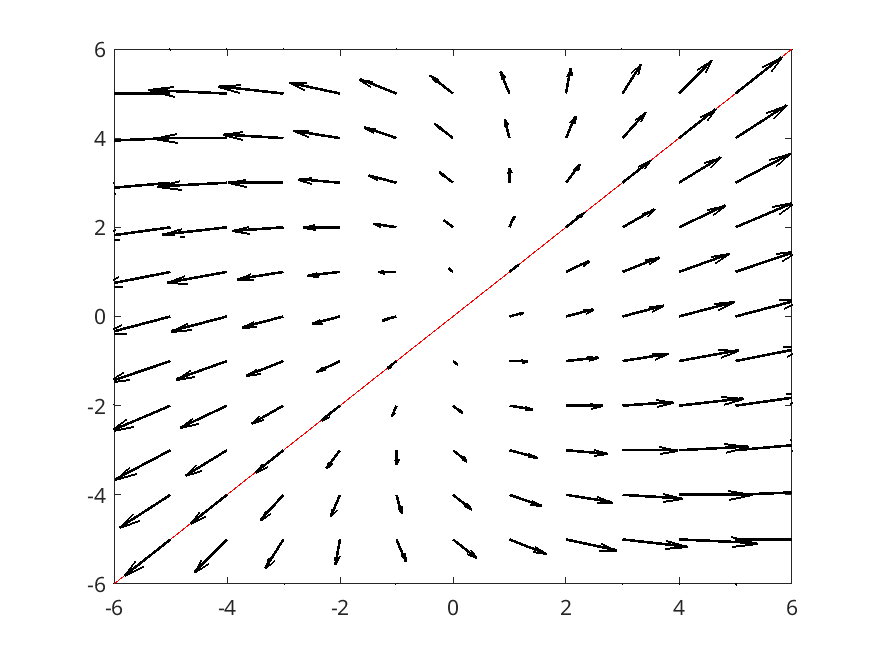
\includegraphics[scale=0.75]{./images/2.png}
		\caption{Фазовый портрет системы}
	\end{figure}	
	
	Видим неустойчивый узел с одним вектором, направленным вдоль $y=x$, а значит, построено верно!
	
	Зададим теперь различные начальные условия (все они будут уходить либо на плюс, либо на минус бесконечность, ведь наша система неустойчива):
	
	\begin{figure}
		\centering
		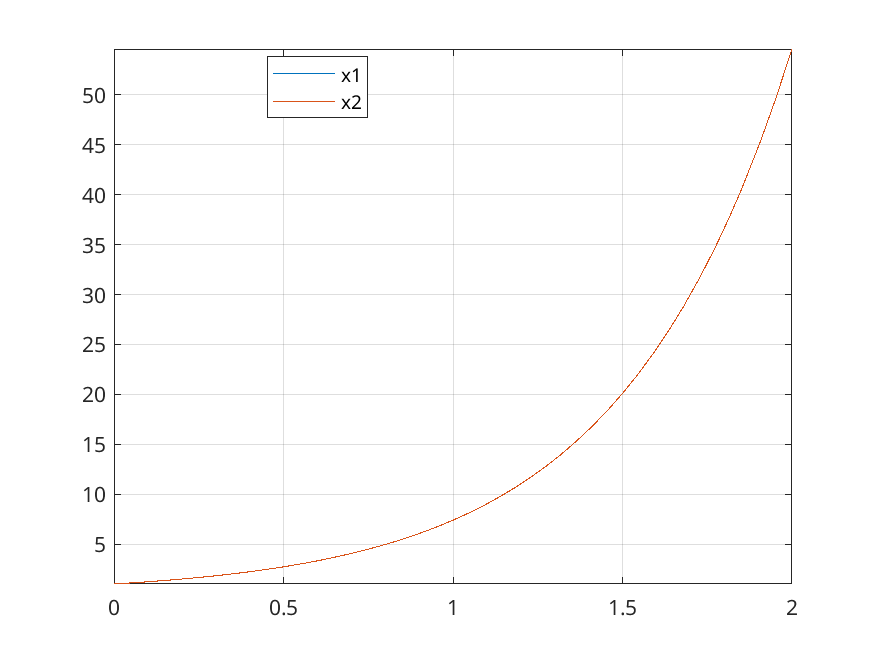
\includegraphics[scale=0.75]{./images/2_1.png}
		\caption{Графики для начальных условий $(1, 1)$}
	\end{figure}
	
	\begin{figure}
		\centering
		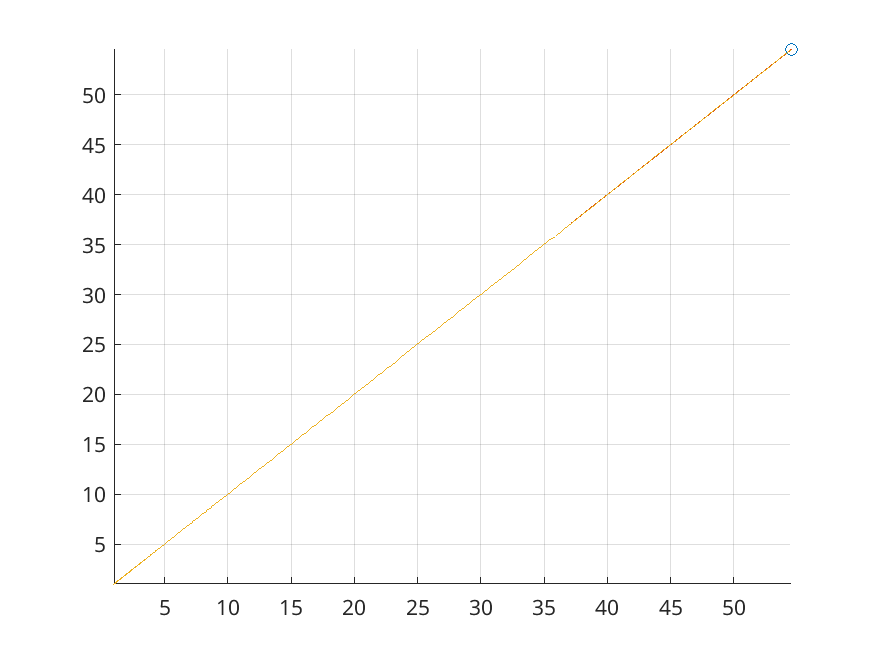
\includegraphics[scale=0.75]{./images/2_comet_1.png}
		\caption{График зависимости $x_2(x_1)$}
	\end{figure}
	
	\begin{figure}
		\centering
		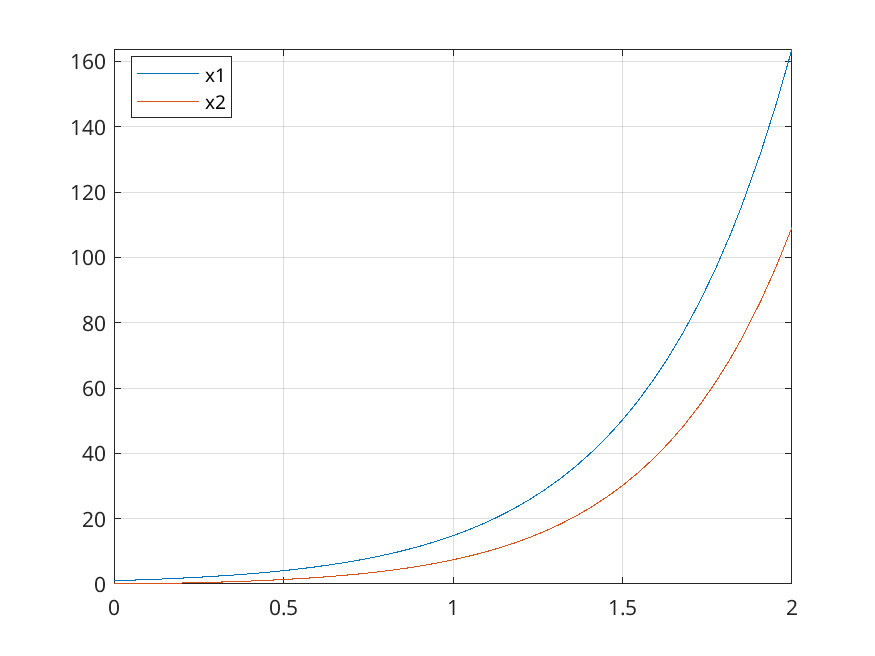
\includegraphics[scale=0.75]{./images/2_2.png}
		\caption{Графики для начальных условий $(1, 0)$}
	\end{figure}
	
	\begin{figure}
		\centering
		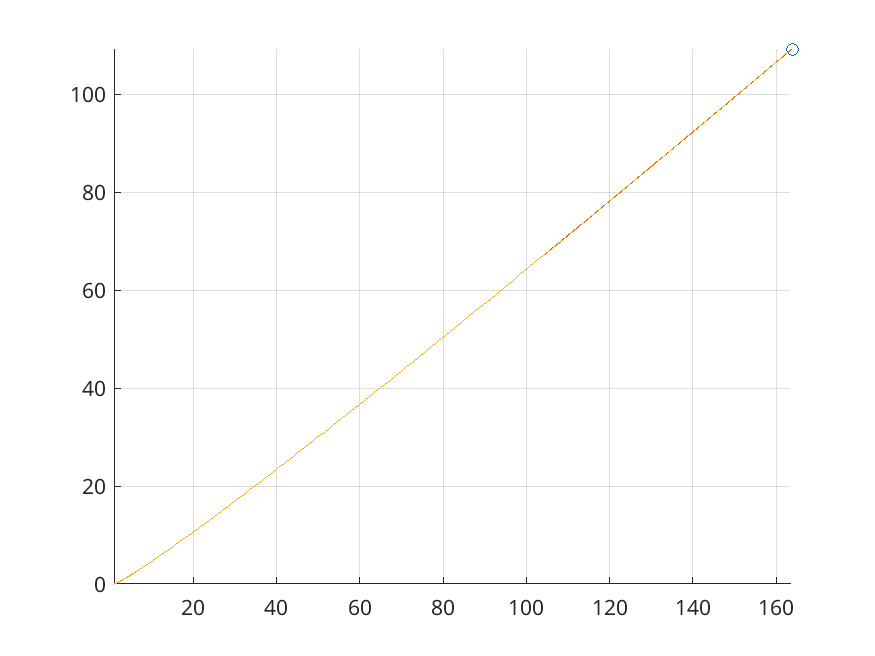
\includegraphics[scale=0.75]{./images/2_comet_2.png}
		\caption{График зависимости $x_2(x_1)$}
	\end{figure}
	
	\begin{figure}
		\centering
		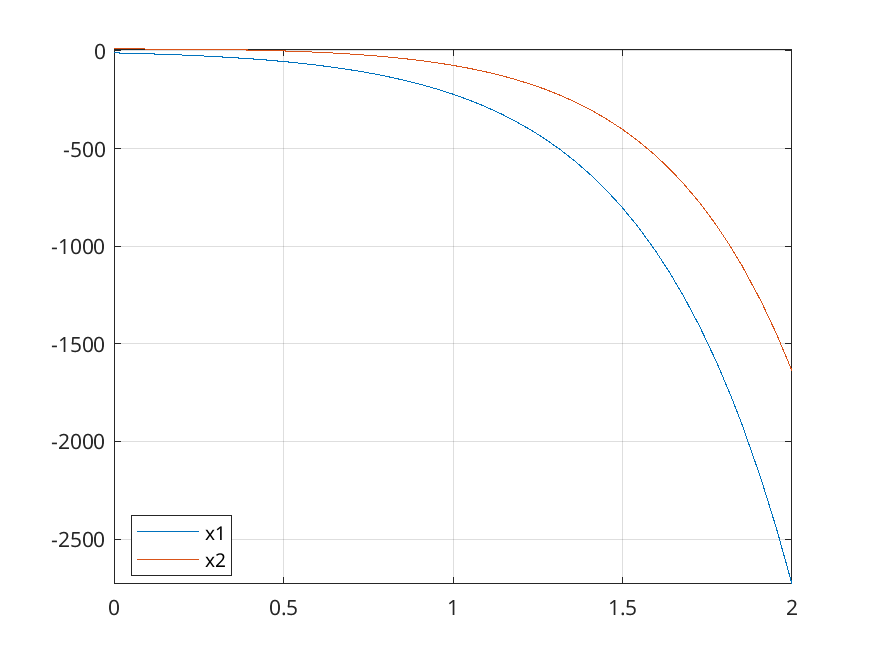
\includegraphics[scale=0.75]{./images/2_3.png}
		\caption{Графики для начальных условий $(-10, 10)$}
	\end{figure}
	
	\begin{figure}
		\centering
		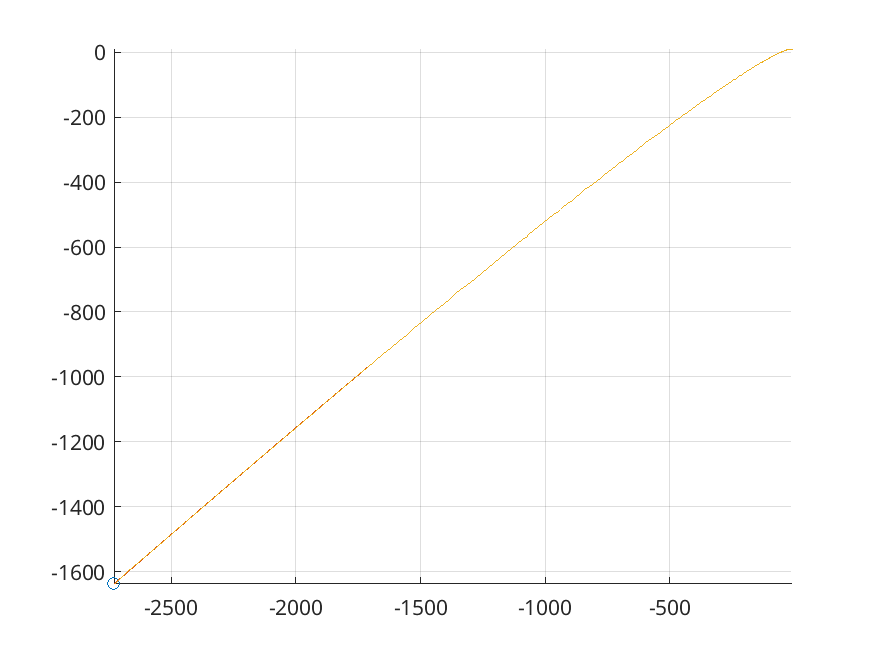
\includegraphics[scale=0.75]{./images/2_comet_3.png}
		\caption{График зависимости $x_2(x_1)$}
	\end{figure}
	
	\pagebreak
	
	\subsection{Особая неустойчивость}
	Хотим получить неуйстойчивую систему, для которой если $x(0)=v_1$, то $\lim\limits_{t\to\infty}x(t)=0$. Этому удовлетворяет система со следующей матрицей:
	\[
	A = \begin{bmatrix}
		\phantom{-}13 & -15 \\
		-18 & \phantom{-}16
	\end{bmatrix}
	\]
	
	
	Собственные вектора - $v_1=\begin{bmatrix}
		1 \\ 1
	\end{bmatrix}, v_2=\begin{bmatrix}
		-5 \\ 6	\end{bmatrix}$; а собственные числа - $\lambda_1=-2$, $\lambda_2=31$. Из общего вида решения систем дифференциальных уравнений очевидно, что матрица полностью удовлетворяет условию.
	
	Векторное поле имеет следующий вид:
	
	\begin{figure}[h]
		\centering
		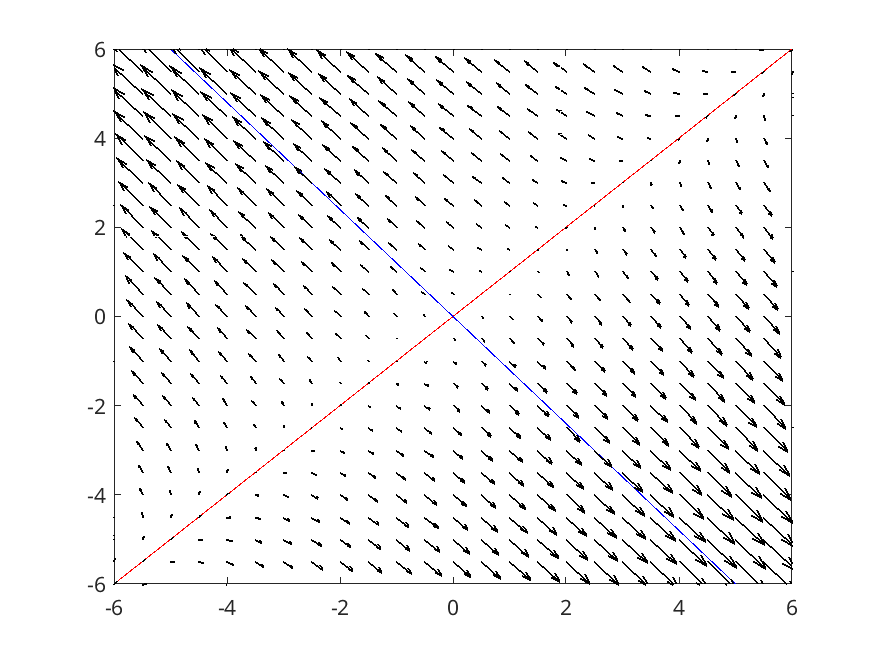
\includegraphics[scale=0.75]{./images/3.png}
		\caption{Фазовый портрет системы}
	\end{figure}
	
	Возле прямой $y=x$ стрелки, завихряясь к $y=-\frac{6}{5}x$, направлены к $(0, 0)$, что говорит о правильности нашего задания системы, а график для начального условия $x(0)=v_1$, приведенный ниже говорит о выполнении условия задания.
	
	Графики для различных начальных условий будут следующими:
	
	\begin{figure}
		\centering
		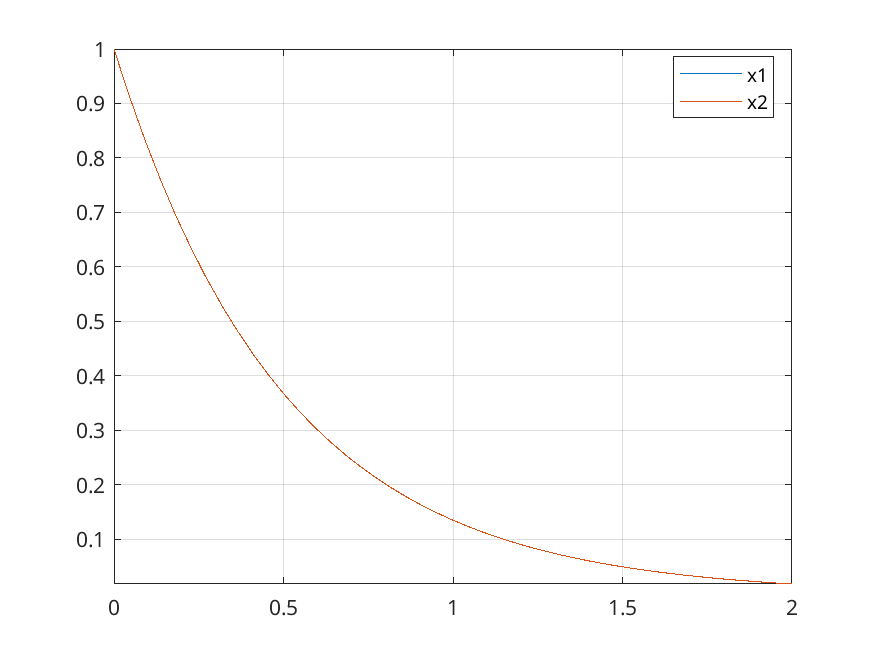
\includegraphics[scale=0.75]{./images/3_1.png}
		\caption{Графики для начальных условий $(1, 1)$}
	\end{figure}
	
	\begin{figure}
		\centering
		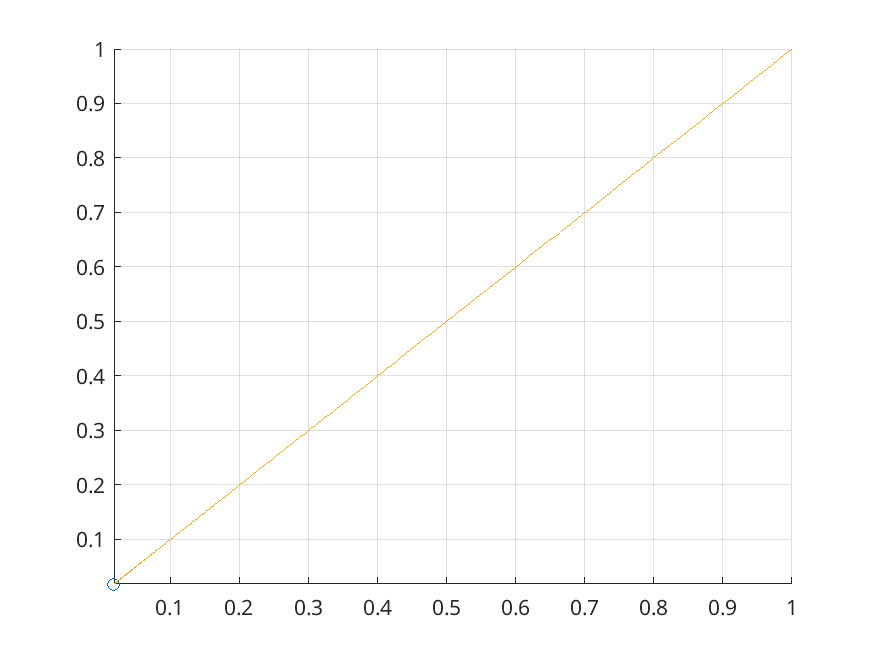
\includegraphics[scale=0.75]{./images/3_comet_1.png}
		\caption{График зависимости $x_2(x_1)$}
	\end{figure}
	
	\begin{figure}
		\centering
		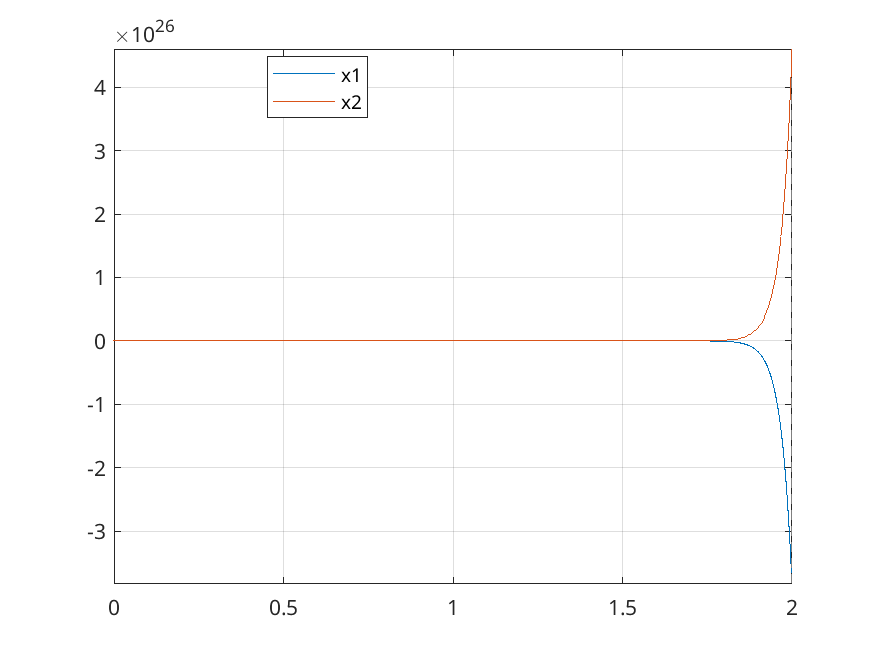
\includegraphics[scale=0.75]{./images/3_2.png}
		\caption{Графики для начальных условий $(2, 3)$}
	\end{figure}
	
	\begin{figure}
		\centering
		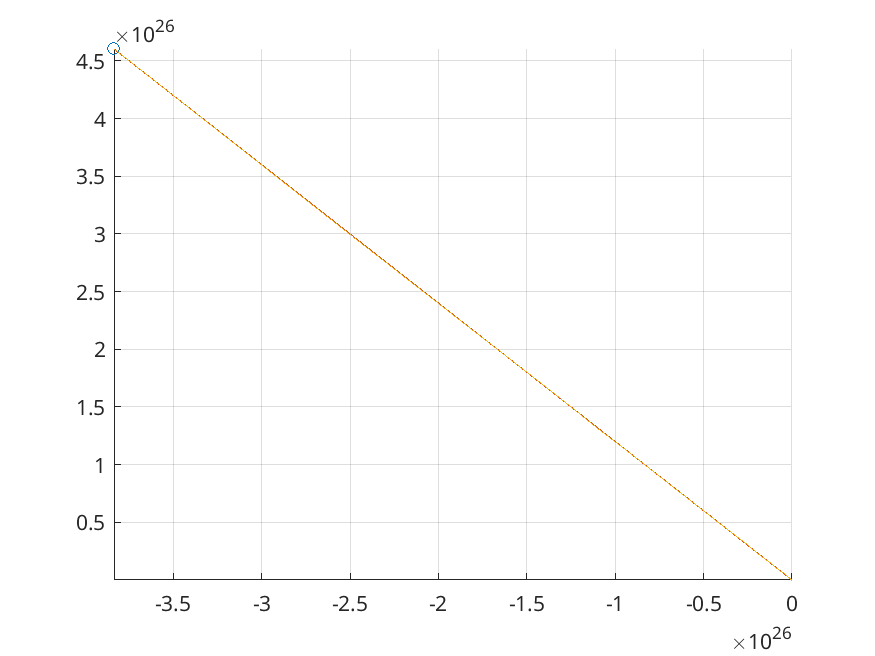
\includegraphics[scale=0.75]{./images/3_comet_2.png}
		\caption{График зависимости $x_2(x_1)$}
	\end{figure}
	
	\begin{figure}
		\centering
		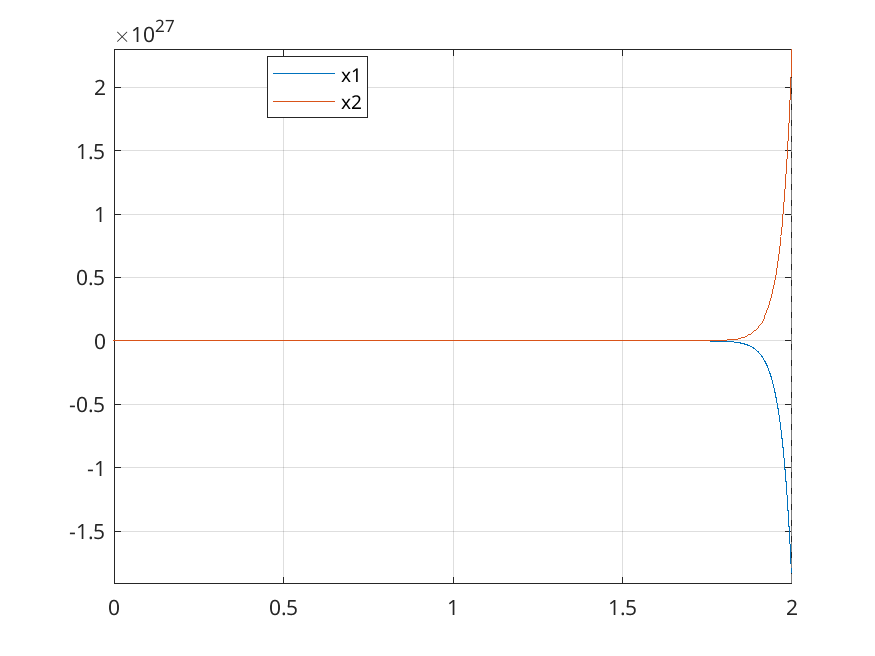
\includegraphics[scale=0.75]{./images/3_3.png}
		\caption{Графики для начальных условий $(-10, -5)$}
	\end{figure}
	
	\begin{figure}
		\centering
		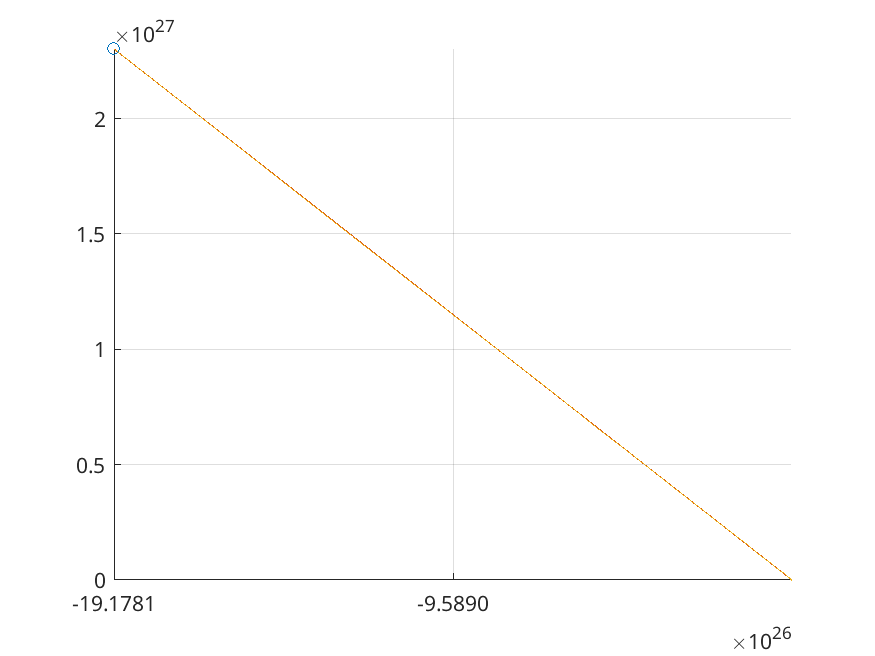
\includegraphics[scale=0.75]{./images/3_comet_3.png}
		\caption{График зависимости $x_2(x_1)$}
	\end{figure}
	
	\pagebreak
	
	\subsection{Асимптотическая устойчивость}
	Необходимо придумать вещественную матрицу, имеющей комплексные собственные вектора вида $v_1 \pm v_2i$. Под это условие подходит система с матрицей
	$$
	A = \begin{bmatrix}
		\phantom{-}5 & \phantom{-}5 \\
		-13 & -9
	\end{bmatrix}
	$$
	
	Собственные вектора - $u_1=\begin{bmatrix}
		1-3i \\ 1+5i
	\end{bmatrix}, u_2=\begin{bmatrix}
	1+3i \\ 1-5i
	\end{bmatrix}$; а собственные значения матрицы - $\lambda_1=-2-4i$, $\lambda_2=-2+4i$. Вещественная часть собственных чисел меньше 0, а значит, имеем ситуацию асимптотической устойчивости, что и требовалось от нас.
	
	Посмотрим на вид нашей системы:
	
	\begin{figure}[h]
		\centering
		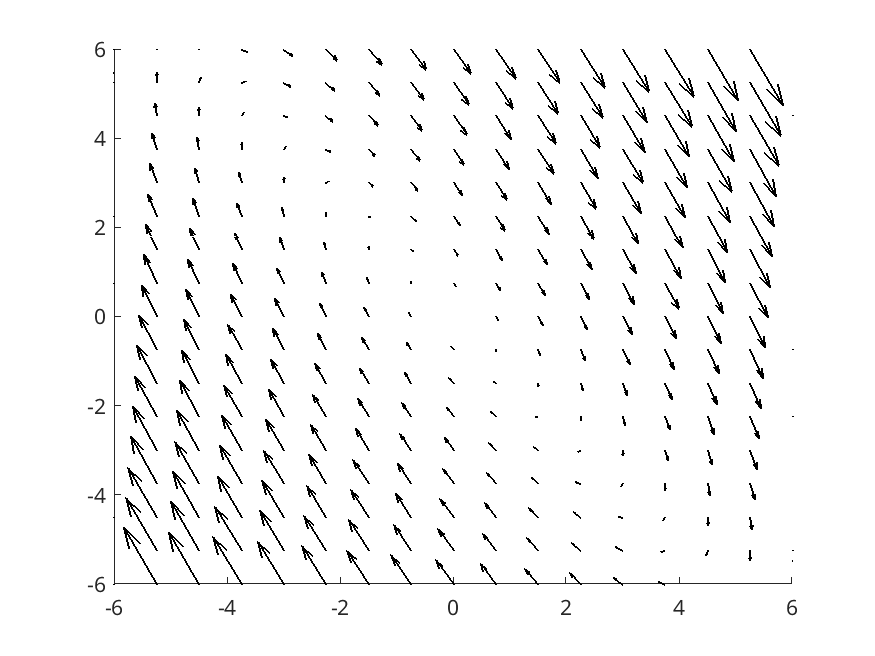
\includegraphics[scale=0.75]{./images/4.png}
		\caption{Фазовый портрет системы}
	\end{figure}
	
	Получается устойчивый фокус, что мы и хотели!
	
	А вот графики для различных начальных условий $x(0)$:
	
	\begin{figure}
		\centering
		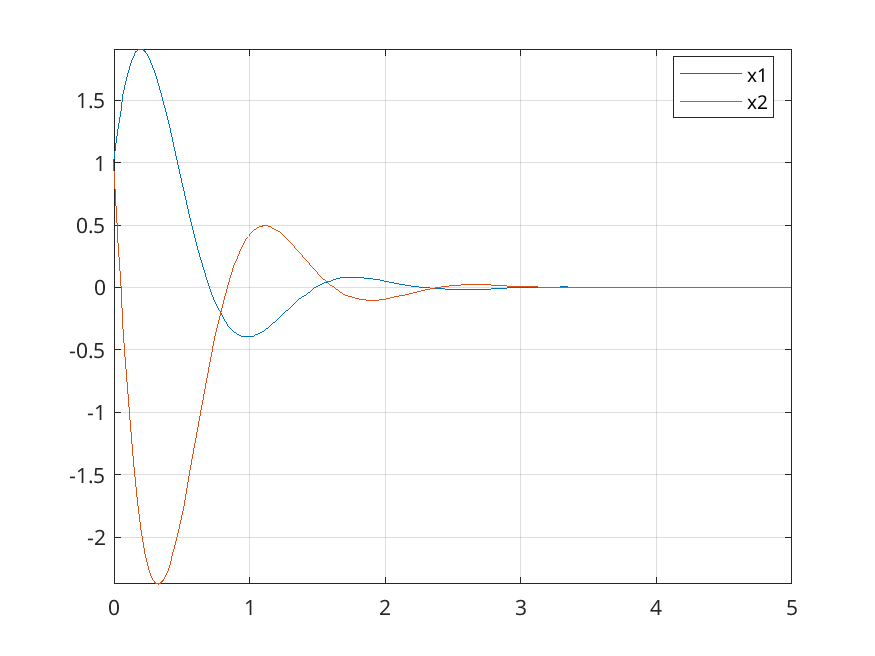
\includegraphics[scale=0.75]{./images/4_1.png}
		\caption{Графики для начальных условий $(1, 1)$}
	\end{figure}
	
	\begin{figure}
		\centering
		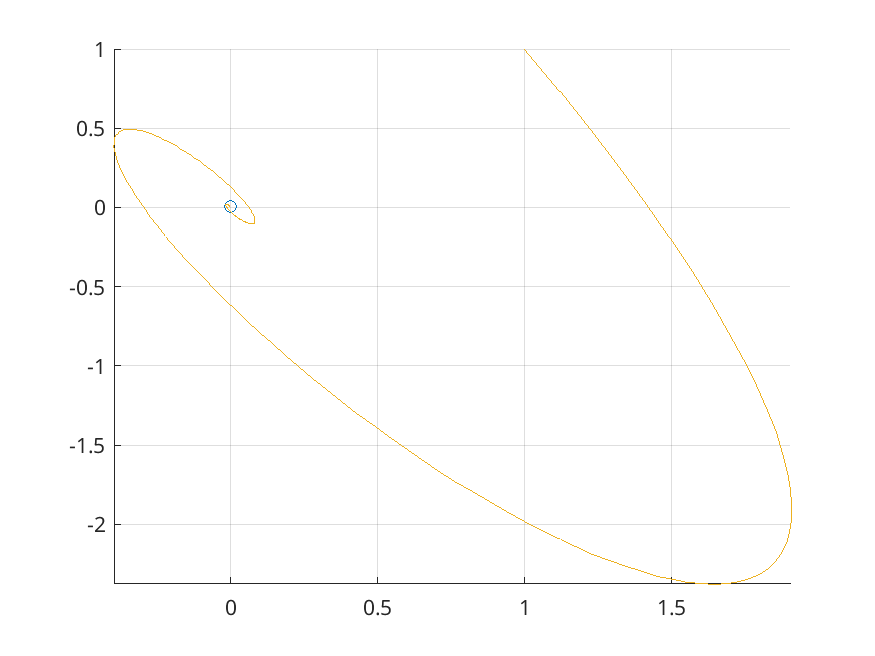
\includegraphics[scale=0.75]{./images/4_comet_1.png}
		\caption{График зависимости $x_2(x_1)$}
	\end{figure}
	
	\begin{figure}
		\centering
		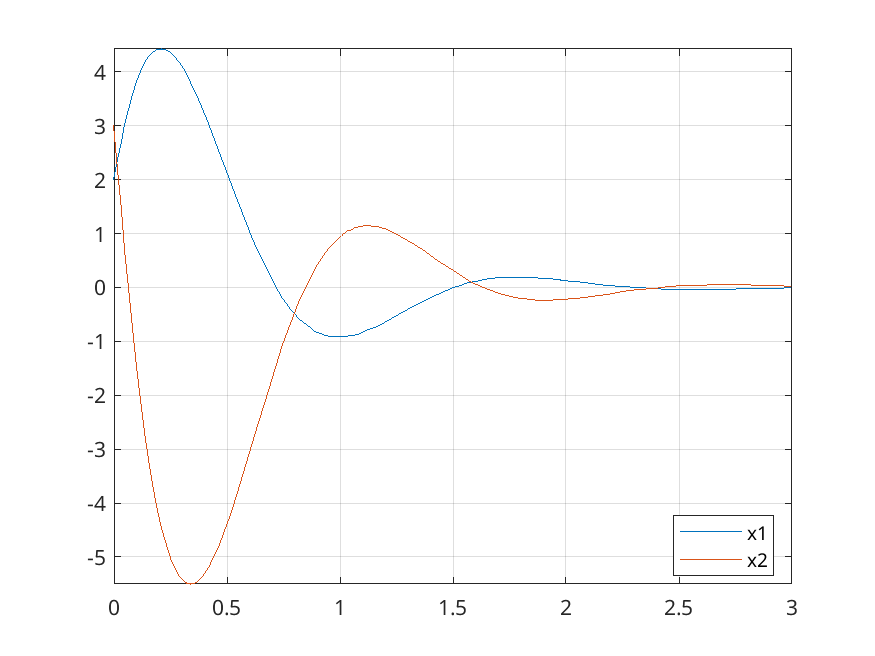
\includegraphics[scale=0.75]{./images/4_2.png}
		\caption{Графики для начальных условий $(2, 3)$}
	\end{figure}
	
	\begin{figure}
		\centering
		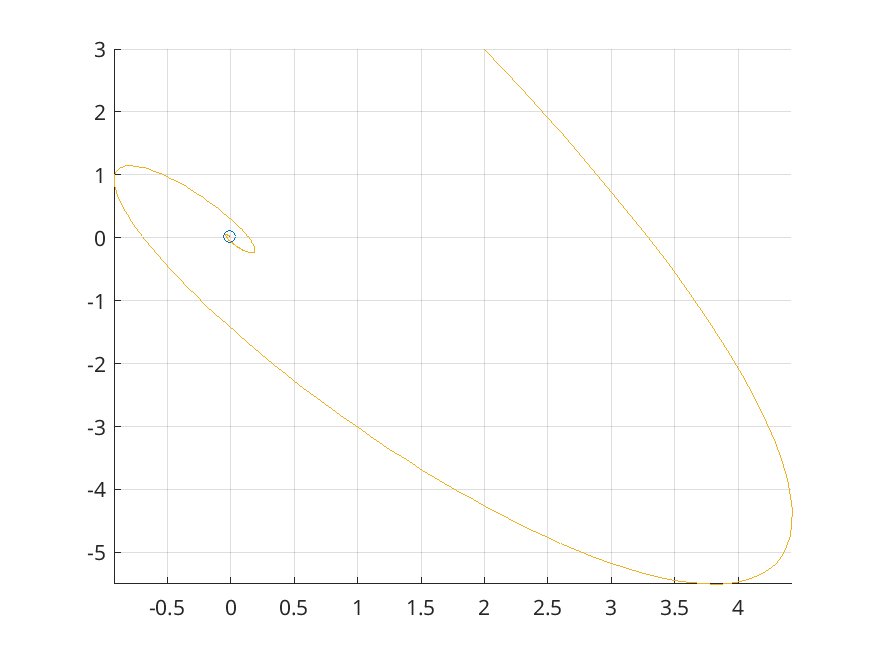
\includegraphics[scale=0.75]{./images/4_comet_2.png}
		\caption{График зависимости $x_2(x_1)$}
	\end{figure}
	
	\begin{figure}
		\centering
		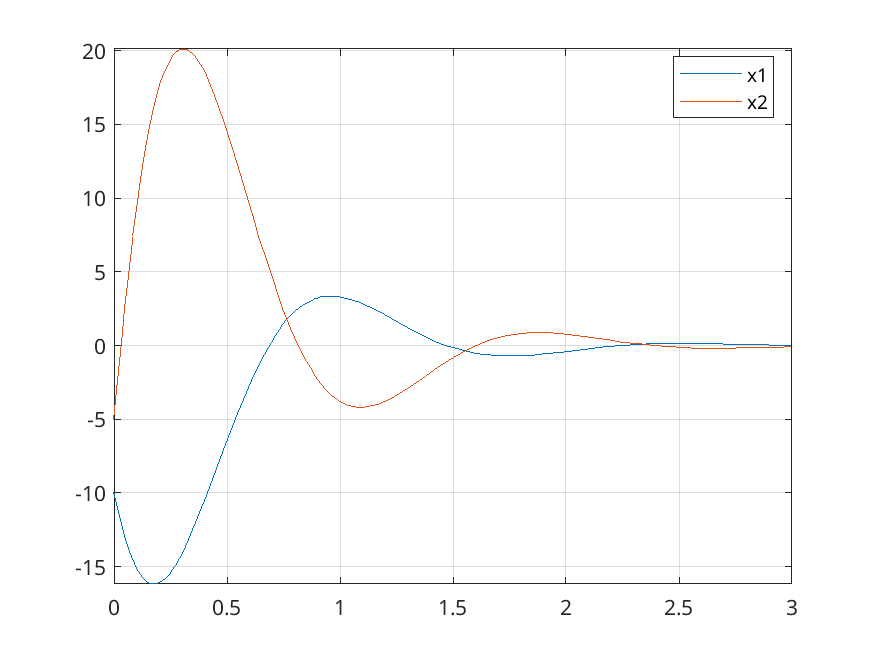
\includegraphics[scale=0.75]{./images/4_3.png}
		\caption{Графики для начальных условий $(-10, -5)$}
	\end{figure}
	
	\begin{figure}
		\centering
		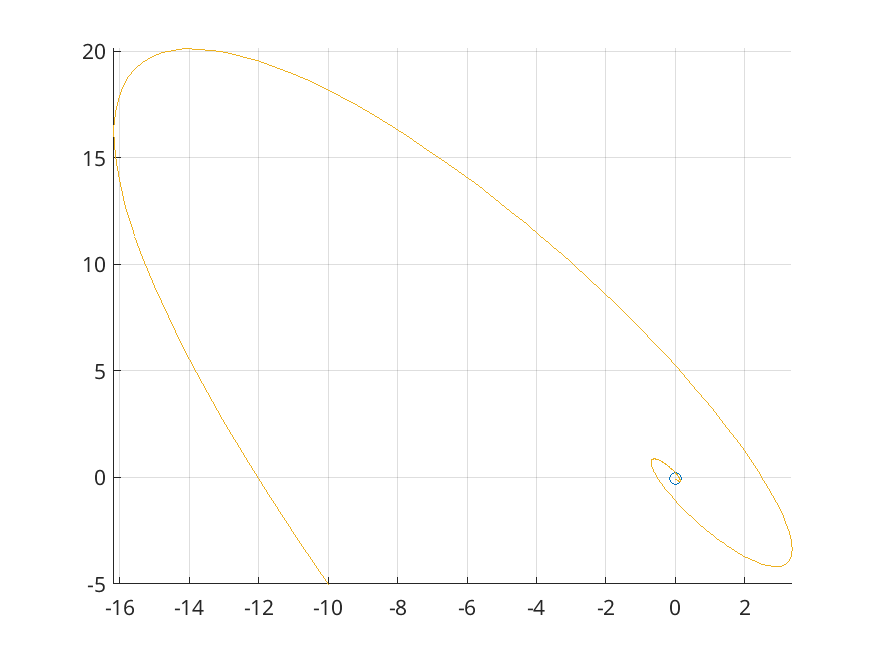
\includegraphics[scale=0.75]{./images/4_comet_3.png}
		\caption{График зависимости $x_2(x_1)$}
	\end{figure}
	
	\pagebreak
	
	\subsection{Неустойчивая система}
	Хотим получить те же собственные вектора, что и в предыдущем примере, только теперь вместе асимптотической устойчивости требуем неустойчивость.
	
	Данному удовлетворяет следующая матрица:
	$$
	A = \begin{bmatrix}
		-5 & -5 \\
		\phantom{-}13 & \phantom{-}9
	\end{bmatrix}
	$$
	
	Собственные вектора - $u_1=\begin{bmatrix}
		1-3i \\ 1+5i
	\end{bmatrix}, u_2=\begin{bmatrix}
		1+3i \\ 1-5i
	\end{bmatrix}$; собственные значения матрицы - $\lambda_1=2-4i$, $\lambda_2=2+4i$. Вещественная часть собственных чисел больше 0, а значит, все траектории уходят в бесконечность.
	
	Посмотрим на графики и убедимся в этом (как бы ни было удивительно, но лишь смена знака даёт нам абсолютно противоположный результат!):
	
	\begin{figure}
		\centering
		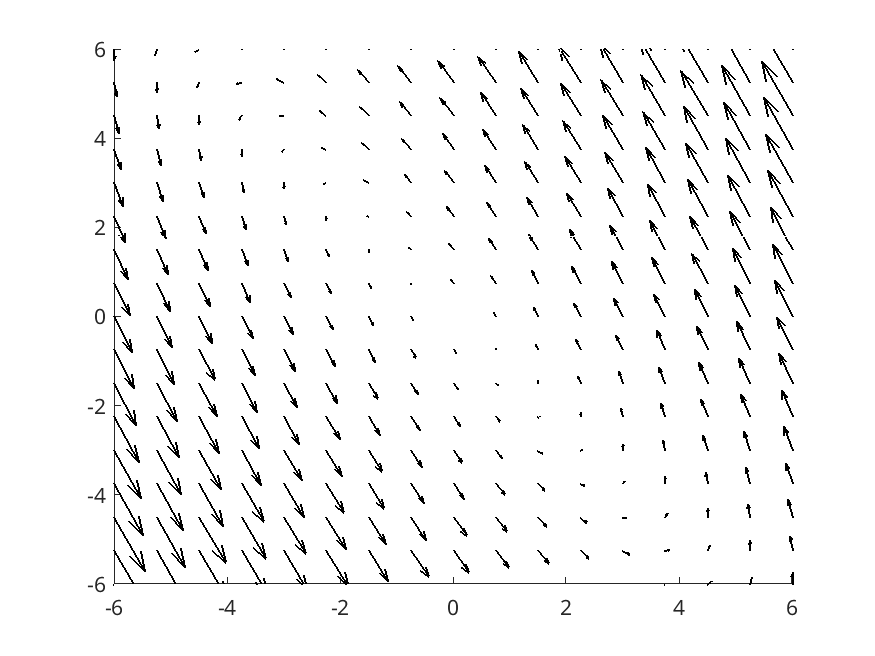
\includegraphics[scale=0.75]{./images/5.png}
		\caption{Фазовый портрет системы}
	\end{figure}
	
	\begin{figure}
		\centering
		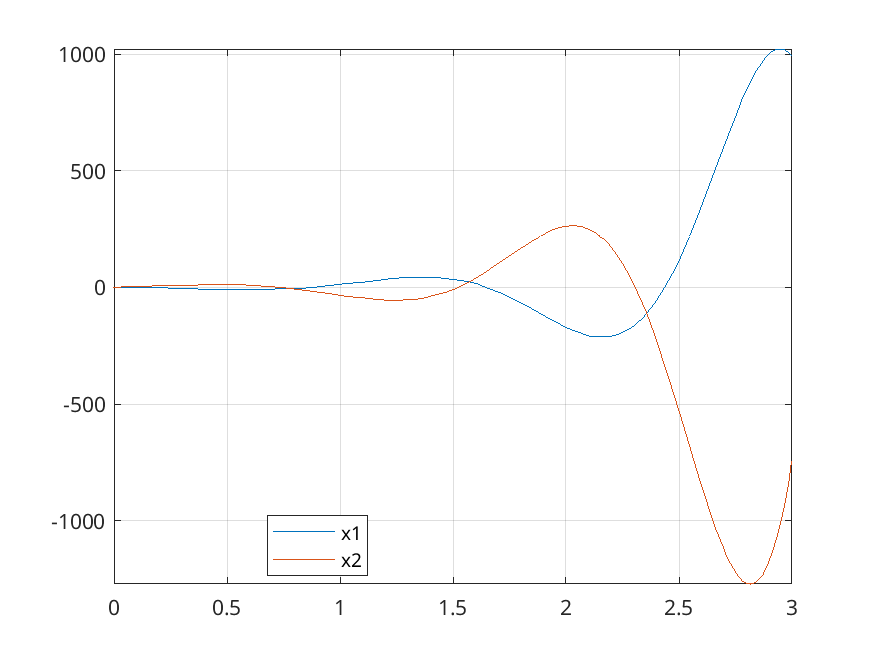
\includegraphics[scale=0.75]{./images/5_1.png}
		\caption{Графики для начальных условий $(1, 1)$}
	\end{figure}
	
	\begin{figure}
		\centering
		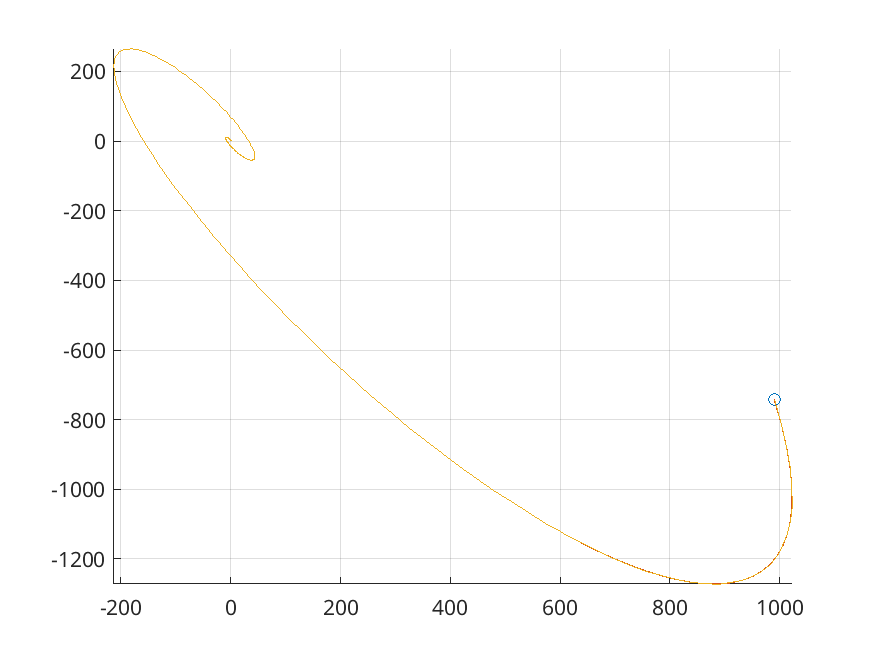
\includegraphics[scale=0.75]{./images/5_comet_1.png}
		\caption{График зависимости $x_2(x_1)$}
	\end{figure}
	
	\begin{figure}
		\centering
		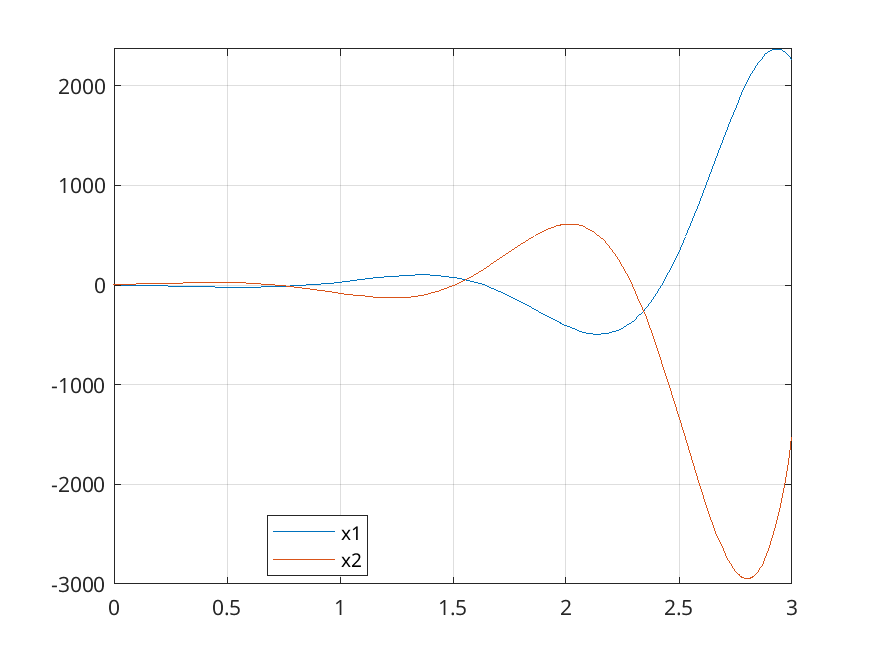
\includegraphics[scale=0.75]{./images/5_2.png}
		\caption{Графики для начальных условий $(2, 3)$}
	\end{figure}
	
	\begin{figure}
		\centering
		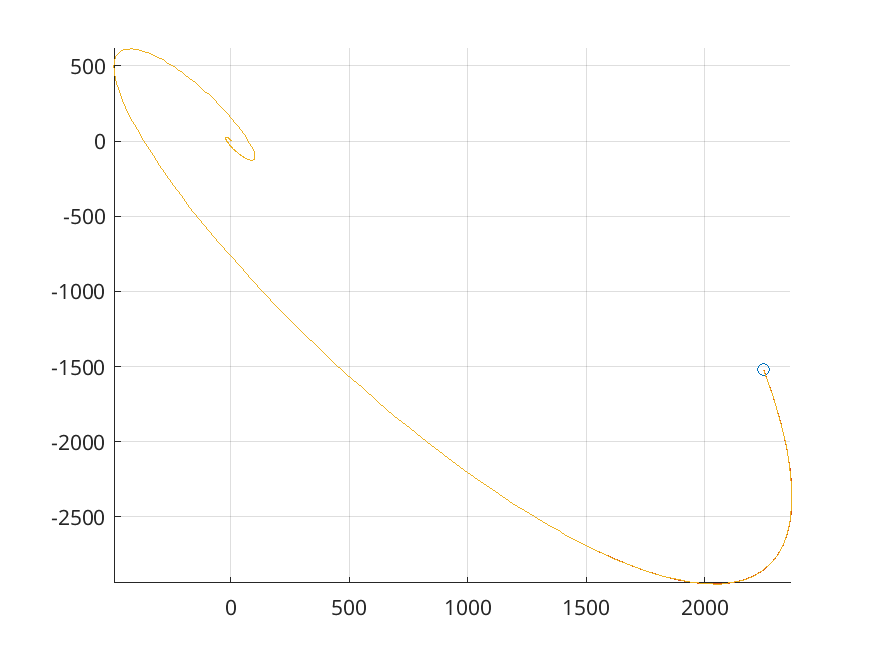
\includegraphics[scale=0.75]{./images/5_comet_2.png}
		\caption{График зависимости $x_2(x_1)$}
	\end{figure}
	
	\begin{figure}
		\centering
		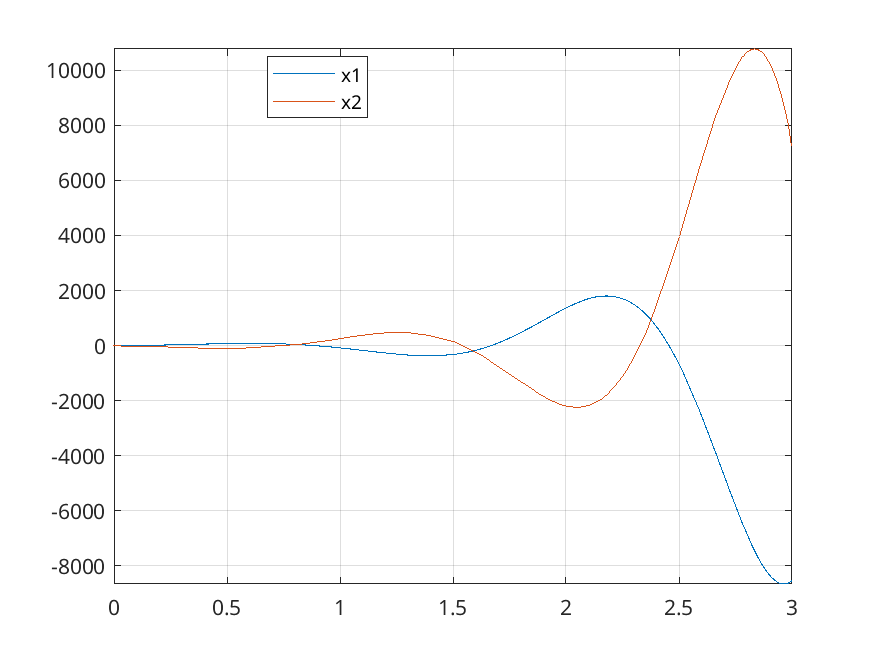
\includegraphics[scale=0.75]{./images/5_3.png}
		\caption{Графики для начальных условий $(-10, -5)$}
	\end{figure}
	
	\begin{figure}
		\centering
		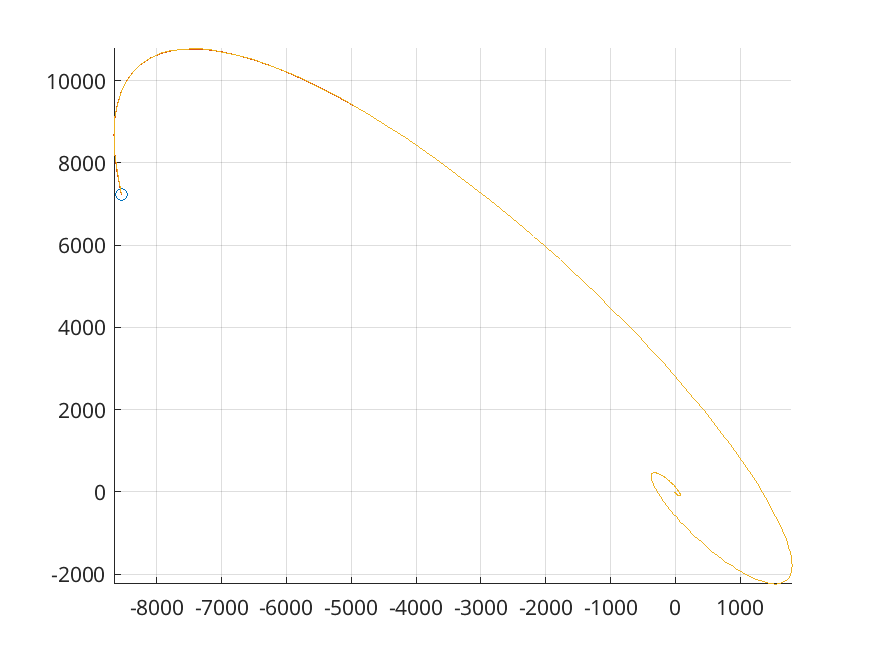
\includegraphics[scale=0.75]{./images/5_comet_3.png}
		\caption{График зависимости $x_2(x_1)$}
	\end{figure}
	
	\pagebreak
	
	\subsection{Устойчивая система}
	При этом матрица системы должна иметь те же собственные вектора, что и в двух предыдущих пунктах.
	
	Рассмотрим систему с матрицей
	
	$$
	A = \begin{bmatrix}
		\phantom{-}7 & \phantom{-}5 \\
		-13 & -7
	\end{bmatrix}
	$$
	
	Она имеет собственные вектора $u_1=\begin{bmatrix}
		1-3i \\ 1+5i
	\end{bmatrix}, u_2=\begin{bmatrix}
		1+3i \\ 1-5i
	\end{bmatrix}$ и собственные числа вида $\lambda_{1, 2}=\pm4i$, вещественная часть которых равна 0, а значит, траектории имеют вид эллипса с центром в $(0, 0)$ (вид устойчивого фокуса).
	
	Убедимся в наших выкладках, построив различные графики:
	
	\begin{figure}[h]
		\centering
		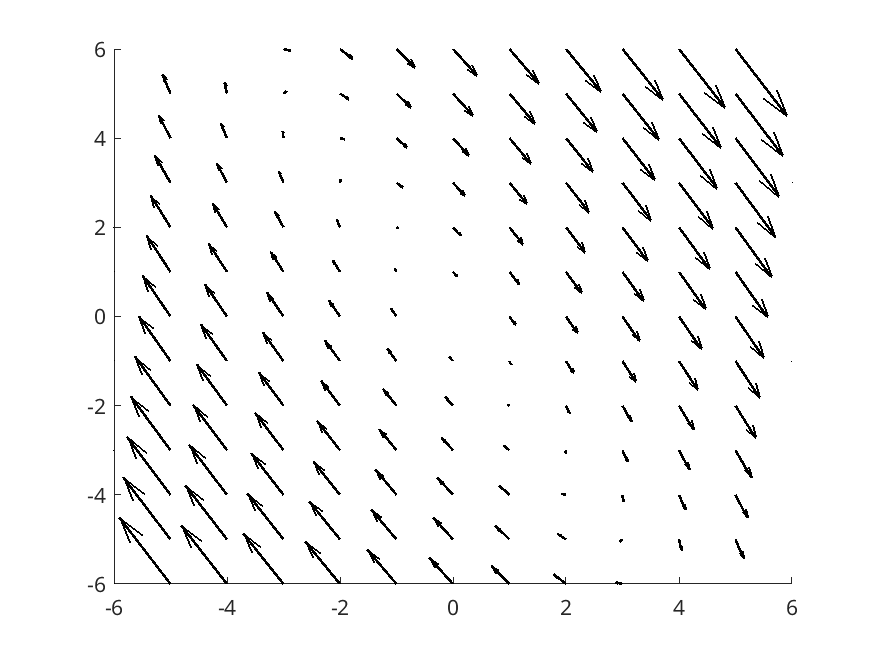
\includegraphics[scale=0.75]{./images/6.png}
		\caption{Фазовый портрет системы}
	\end{figure}
	
	\begin{figure}
		\centering
		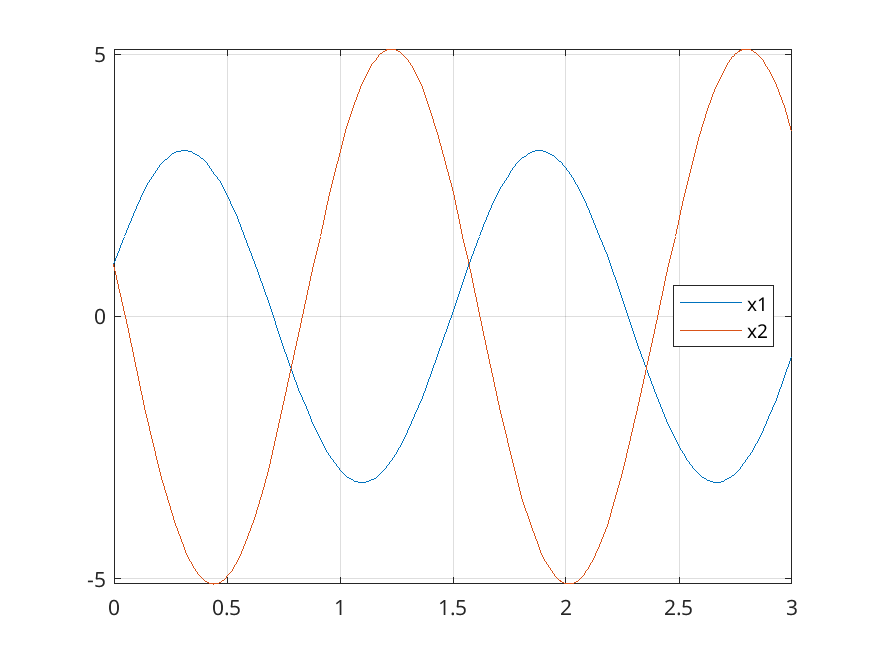
\includegraphics[scale=0.75]{./images/6_1.png}
		\caption{Графики для начальных условий $(1, 1)$}
	\end{figure}
	
	\begin{figure}
		\centering
		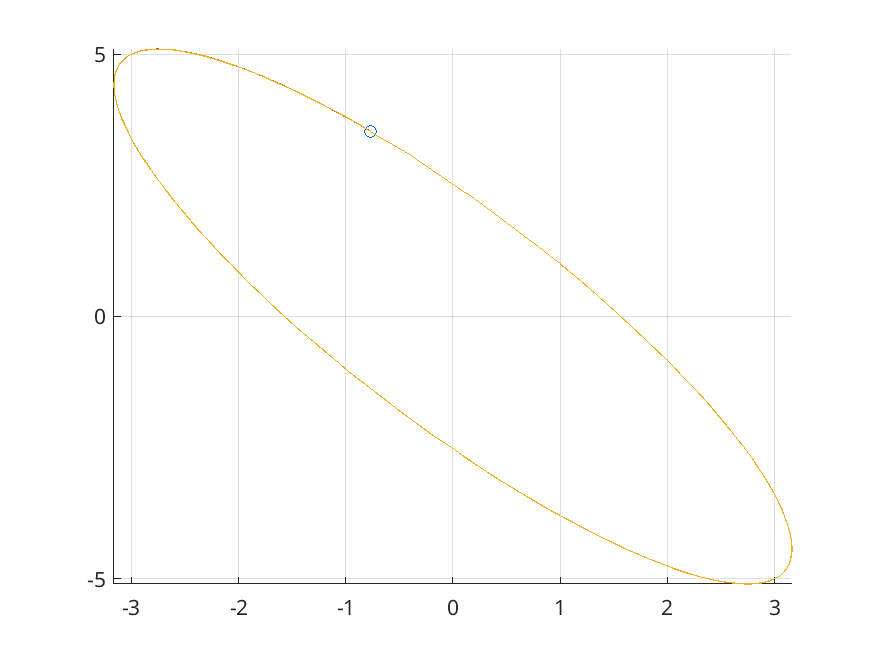
\includegraphics[scale=0.75]{./images/6_comet_1.png}
		\caption{График зависимости $x_2(x_1)$}
	\end{figure}
	
	\begin{figure}
		\centering
		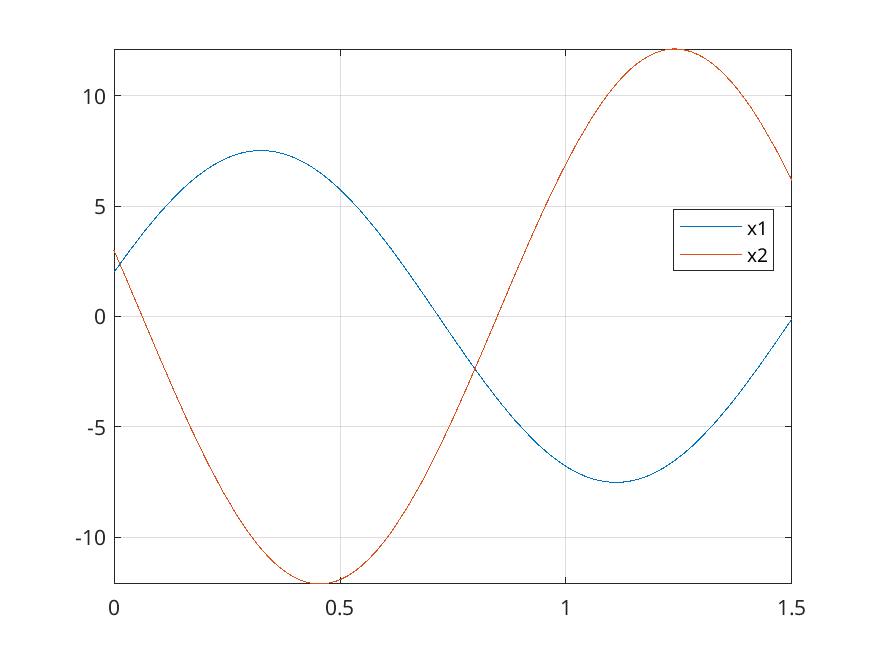
\includegraphics[scale=0.75]{./images/6_2.png}
		\caption{Графики для начальных условий $(2, 3)$}
	\end{figure}
	
	\begin{figure}
		\centering
		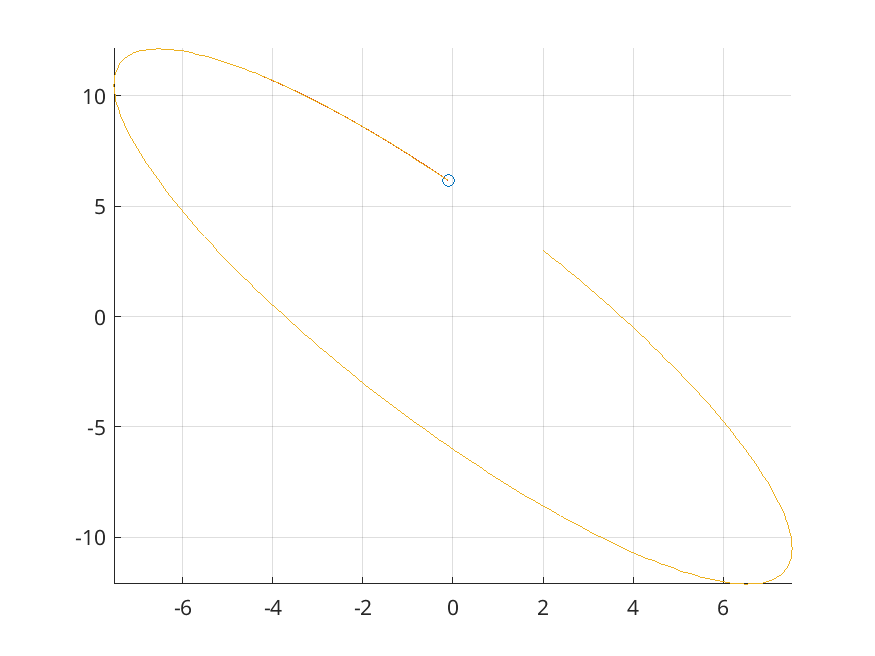
\includegraphics[scale=0.75]{./images/6_comet_2.png}
		\caption{График зависимости $x_2(x_1)$}
	\end{figure}
	
	\begin{figure}
		\centering
		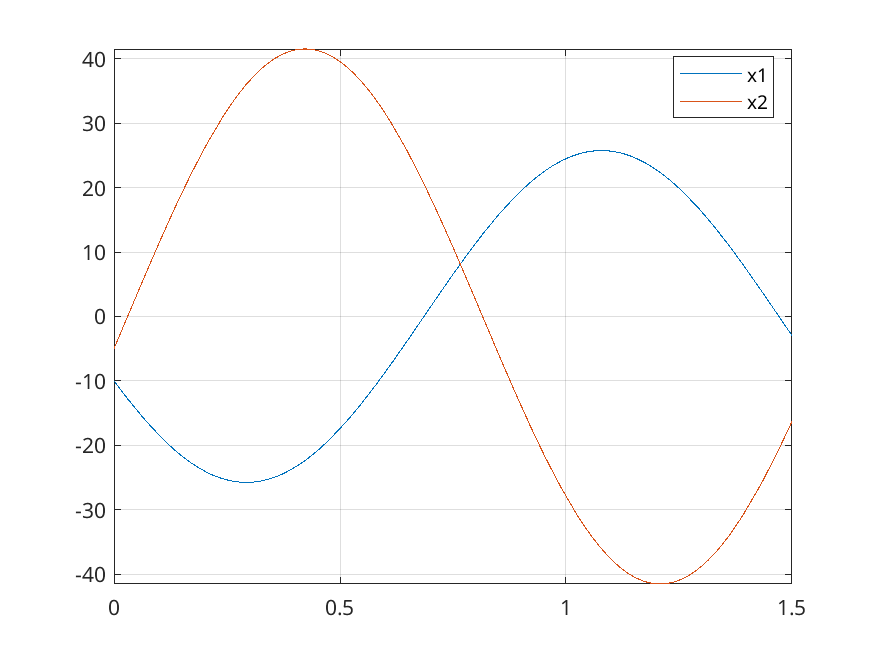
\includegraphics[scale=0.75]{./images/6_3.png}
		\caption{Графики для начальных условий $(-10, -5)$}
	\end{figure}
	
	\begin{figure}
		\centering
		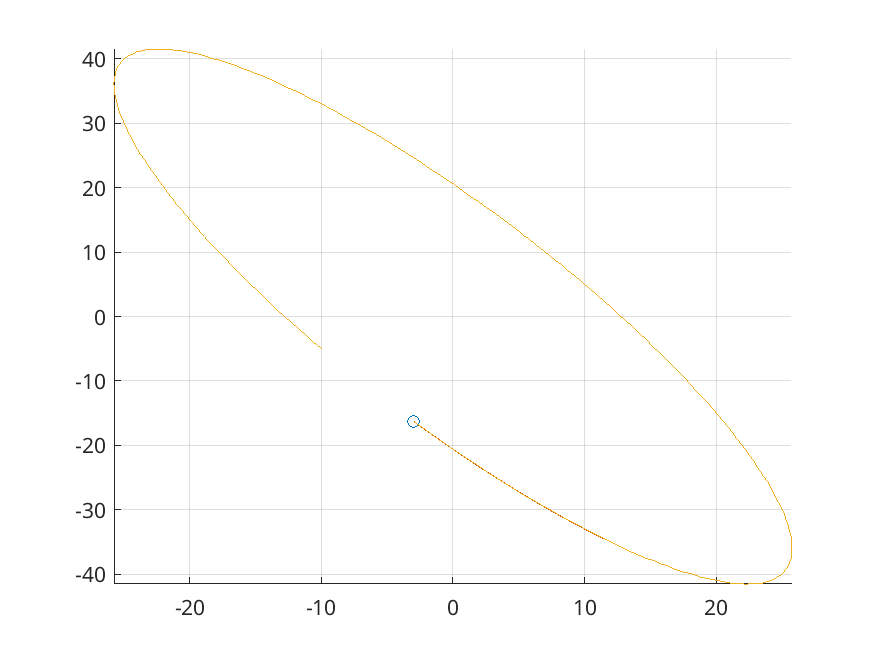
\includegraphics[scale=0.75]{./images/6_comet_3.png}
		\caption{График зависимости $x_2(x_1)$}
	\end{figure}
	
	\pagebreak
	
	
	\section{Изучаем и визуализируем дискретное}
	Здесь мы по большей части отталкиваемся именно от характеристического уравнения, ведь задания связаны с собственными числами систем. Также важно, чтобы наши матрицы не были диагональными, ведь тогда всё получается совсем просто...
	
	\subsection{Собственные значения $\lambda_{1,2}=-1$}
	Матрица
	$$
	A = \begin{bmatrix}
		-1 & \phantom{-}0 \\
		\phantom{-}1 & -1
	\end{bmatrix}
	$$
	
	имеет именно такие собственные числа!
	
	Её визуализация:
	\begin{figure}[h]
		\centering
		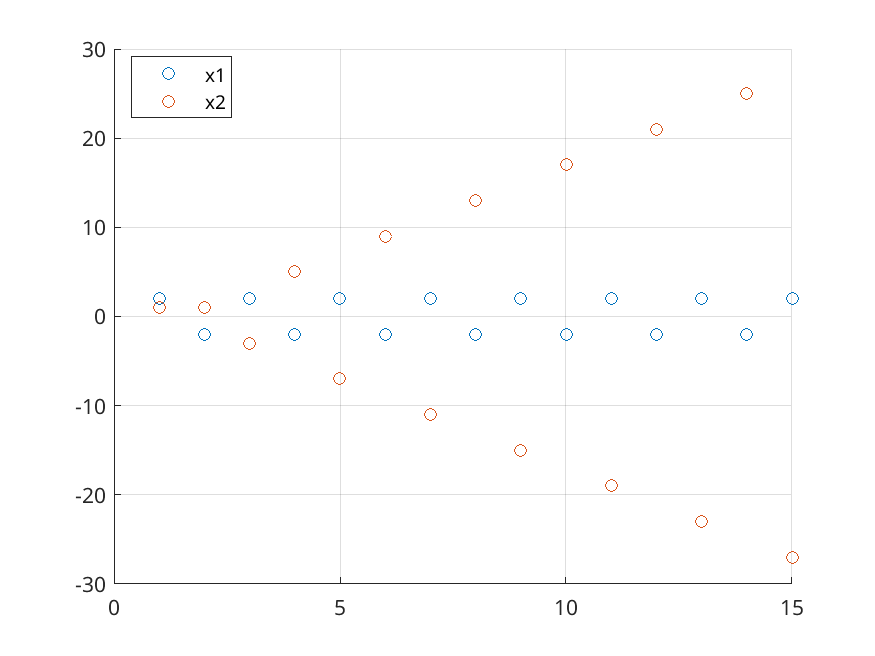
\includegraphics[scale=0.75]{./images/disk1.png}
		\caption{Графики $x_1$ и $x_2$ для начального условия $(2, 1)$}
	\end{figure}
	
	Далее, дабы не нагружать и так большой файл бессмысленным и повторяющимся текстом, будет просто приводится матрица, удовлетворяющая условию, а также её визуализация для различных начальных значений.
	
	
	\subsection{Собственные значения $\lambda_{1,2}=-\frac{1}{\sqrt{2}}\pm\frac{1}{\sqrt{2}}i$}
	Получаем матрицу
	$$
	A = \begin{bmatrix}
		-\frac{1}{\sqrt{2}} & -1 \\
		\phantom{-}\frac{1}{2} & -\frac{1}{\sqrt{2}}
	\end{bmatrix}
	$$
	
	Её визуализация:
	\begin{figure}[h]
		\centering
		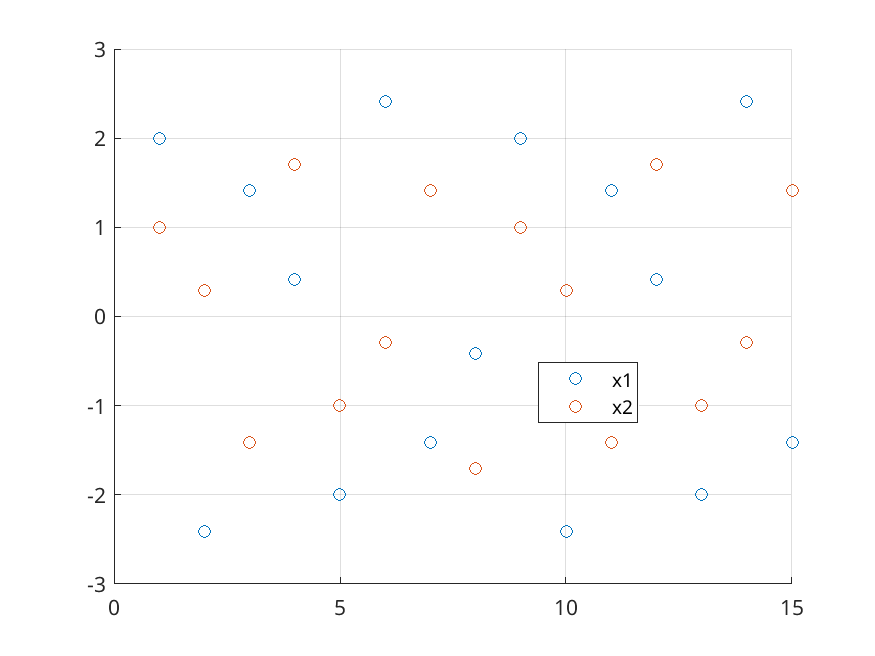
\includegraphics[scale=0.75]{./images/disk2.png}
		\caption{Графики $x_1$ и $x_2$ для начального условия $(2, 1)$}
	\end{figure}
	
	\subsection{Собственные значения $\lambda_{1,2}=\pm i$}
	Получаем матрицу
	$$
	A = \begin{bmatrix}
		0 & -1 \\
		1 & \phantom{-}0
	\end{bmatrix}
	$$
	\pagebreak
	
	Её визуализация:
	\begin{figure}[h]
		\centering
		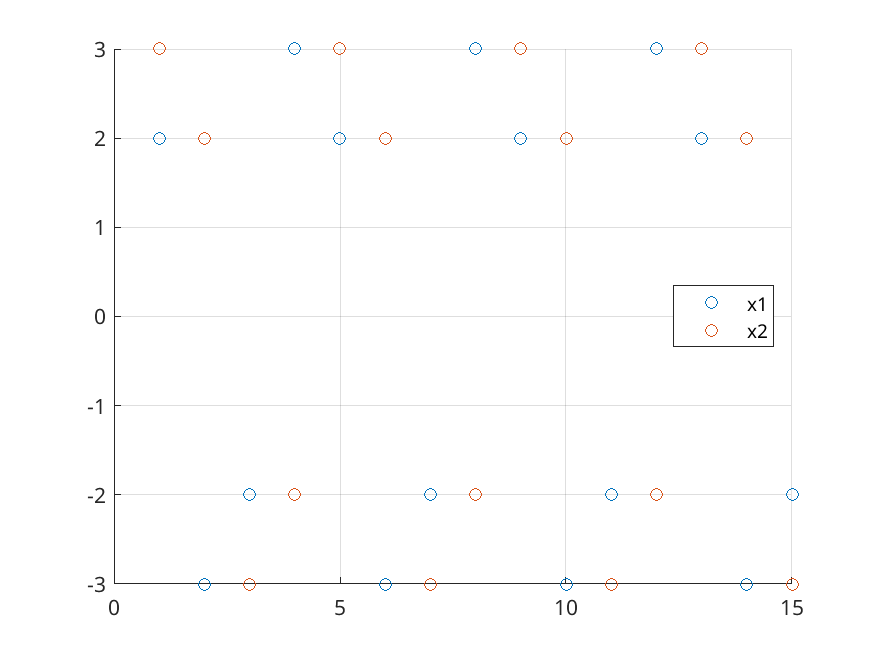
\includegraphics[scale=0.75]{./images/disk3.png}
		\caption{Графики $x_1$ и $x_2$ для начального условия $(2, 3)$}
	\end{figure}
	
	\subsection{Собственные значения $\lambda_{1,2}=\frac{1}{\sqrt{2}}\pm\frac{1}{\sqrt{2}}i$}
	Матрица
	$$
	A = \begin{bmatrix}
		\frac{1}{\sqrt{2}} & -1 \\
		\frac{1}{2} & \phantom{-}\frac{1}{\sqrt{2}}
	\end{bmatrix}
	$$
	\pagebreak
	
	Её визуализация:
	\begin{figure}[h]
		\centering
		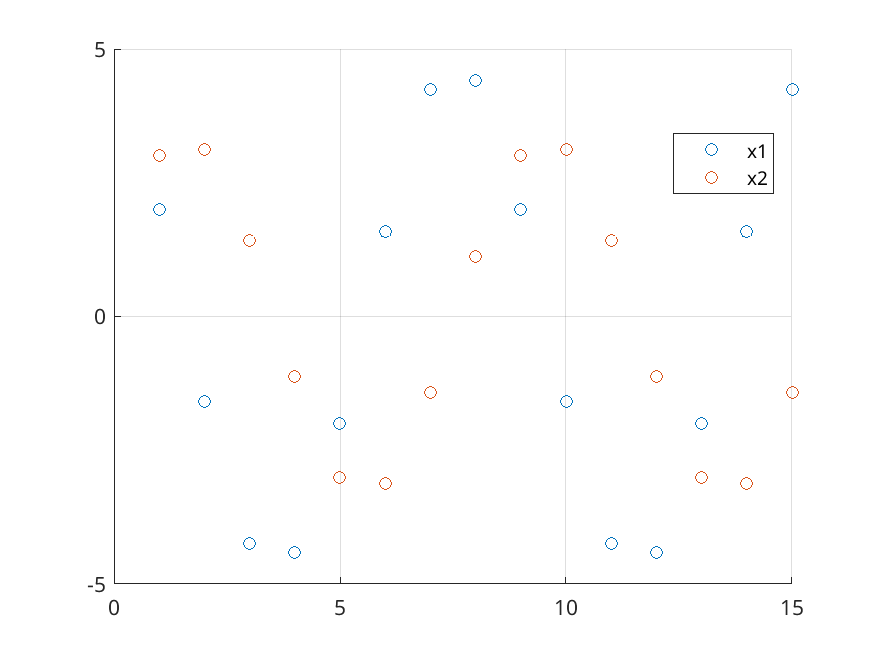
\includegraphics[scale=0.75]{./images/disk4.png}
		\caption{Графики $x_1$ и $x_2$ для начального условия $(2, 3)$}
	\end{figure}
	
	\subsection{Собственные значения $\lambda_{1,2}=1$}
	Получим матрицу из сингулярного разложения
	$$
	A = \begin{bmatrix}
		2 & 4 \\
		3 & 5
	\end{bmatrix}
	\begin{bmatrix}
		1 & 1 \\
		0 & 1
	\end{bmatrix}
	\begin{bmatrix}
		2 & 4 \\
		3 & 5
	\end{bmatrix}^{-1}
	=
	\begin{bmatrix}
		4 & -2 \\
		\frac{9}{2} & -2
	\end{bmatrix}
	$$
	
	\pagebreak
	Визуализация будет следующей:
	\begin{figure}[h]
		\centering
		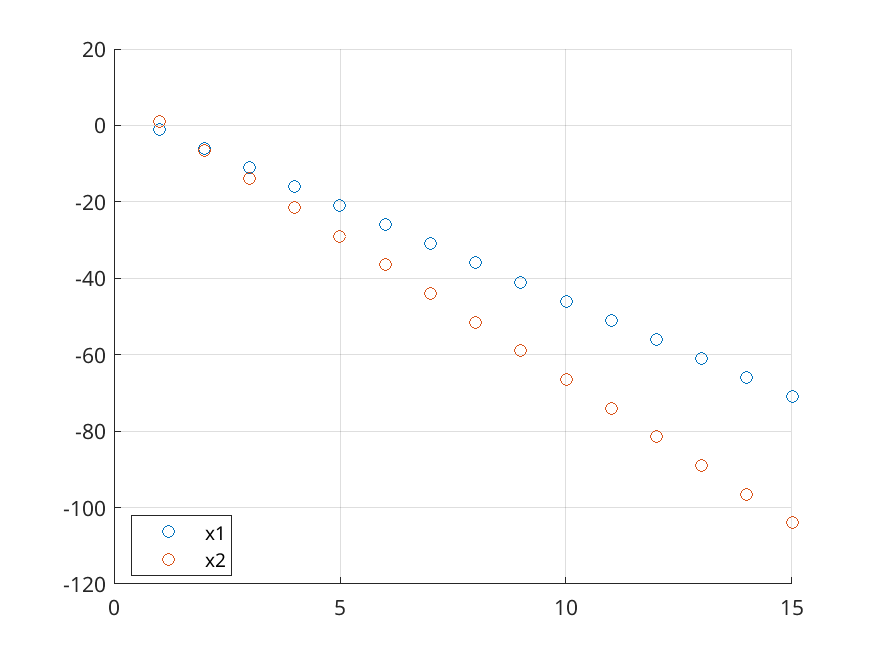
\includegraphics[scale=0.75]{./images/disk5.png}
		\caption{Графики $x_1$ и $x_2$ для начального условия $(-1, 1)$}
	\end{figure}
	
	\subsection{Собственные значения $\lambda_{1,2}=-c=-\frac{1}{5}$}
	То есть качестве константы $c$ взята дробь $\frac{1}{5}$.
	
	Получим матрицу из сингулярного разложения
	$$
	A = \begin{bmatrix}
		5 & 6 \\
		7 & 8
	\end{bmatrix}
	\begin{bmatrix}
		-\frac{1}{5} & \phantom{-}1 \\
		\phantom{-}0 & -\frac{1}{5}
	\end{bmatrix}
	\begin{bmatrix}
		5 & 6 \\
		7 & 8
	\end{bmatrix}^{-1}
	=
	\begin{bmatrix}
		\frac{173}{10} & -\frac{25}{2} \\ \\
		\frac{49}{2} & -\frac{177}{10}
	\end{bmatrix}
	$$
	
	\pagebreak
	Её визуализация:
	\begin{figure}[h]
		\centering
		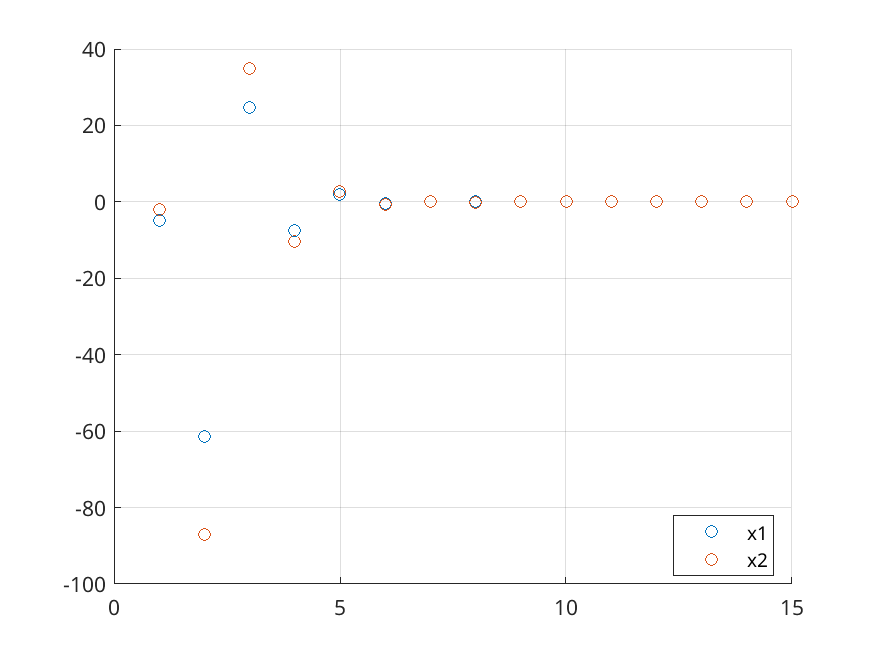
\includegraphics[scale=0.75]{./images/disk6.png}
		\caption{Графики $x_1$ и $x_2$ для начального условия $(-5, -2)$}
	\end{figure}
	
	\subsection{Собственные значения $\lambda_{1,2}=\pm ic=\pm\frac{i}{5}$}
	Матрица:
	$$
	A = \begin{bmatrix}
		0 & -\frac{1}{5} \\
		\frac{1}{5} & \phantom{-}0
	\end{bmatrix}
	$$
	
	\pagebreak
	Её визуализация:
	\begin{figure}[h]
		\centering
		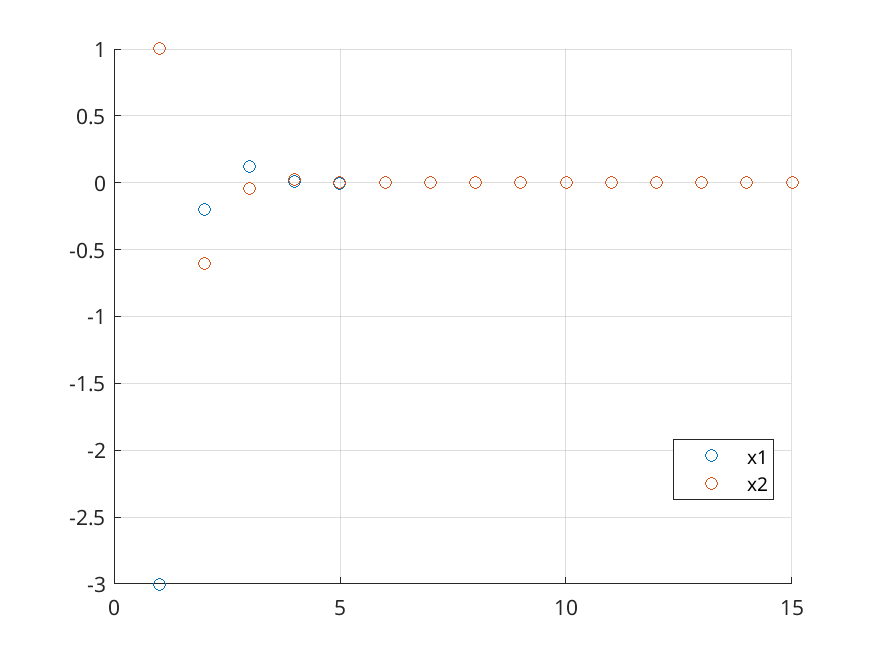
\includegraphics[scale=0.75]{./images/disk7.png}
		\caption{Графики $x_1$ и $x_2$ для начального условия $(-3, 1)$}
	\end{figure}
	
	\subsection{Собственные значения $\lambda_{1,2}=c=\frac{1}{5}$}
	Матрица:
	$$
	A = \begin{bmatrix}
		\frac{21}{5} & -2 \\
		8 & -\frac{19}{5}
	\end{bmatrix}
	$$
	
	\pagebreak
	Её визуализация:
	\begin{figure}[h]
		\centering
		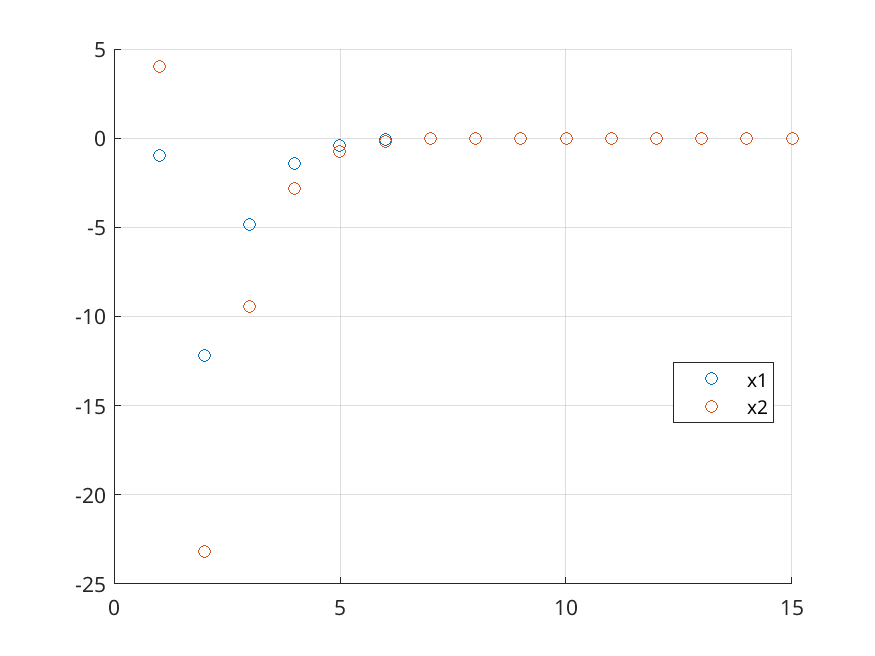
\includegraphics[scale=0.75]{./images/disk8.png}
		\caption{Графики $x_1$ и $x_2$ для начального условия $(-1, 4)$}
	\end{figure}
	
	
	\subsection{Собственные значения $\lambda_{1,2}=-d=-\frac{9}{8}$}
	То есть качестве константы $d$ взята дробь $\frac{9}{8}>1$.
	
	Получим матрицу из сингулярного разложения
	$$
	A = \begin{bmatrix}
		2 & 8 \\
		7 & 5
	\end{bmatrix}
	\begin{bmatrix}
		-\frac{9}{8} & \phantom{-}23 \\
		\phantom{-}0 & -\frac{9}{8}
	\end{bmatrix}
	\begin{bmatrix}
		2 & 8 \\
		7 & 5
	\end{bmatrix}^{-1}
	=
	\begin{bmatrix}
		\frac{47}{8} & -2 \\ \\
		\frac{49}{2} & -\frac{65}{8}
	\end{bmatrix}
	$$
	
	\pagebreak
	Визуализация будет следующей:
	\begin{figure}[h]
		\centering
		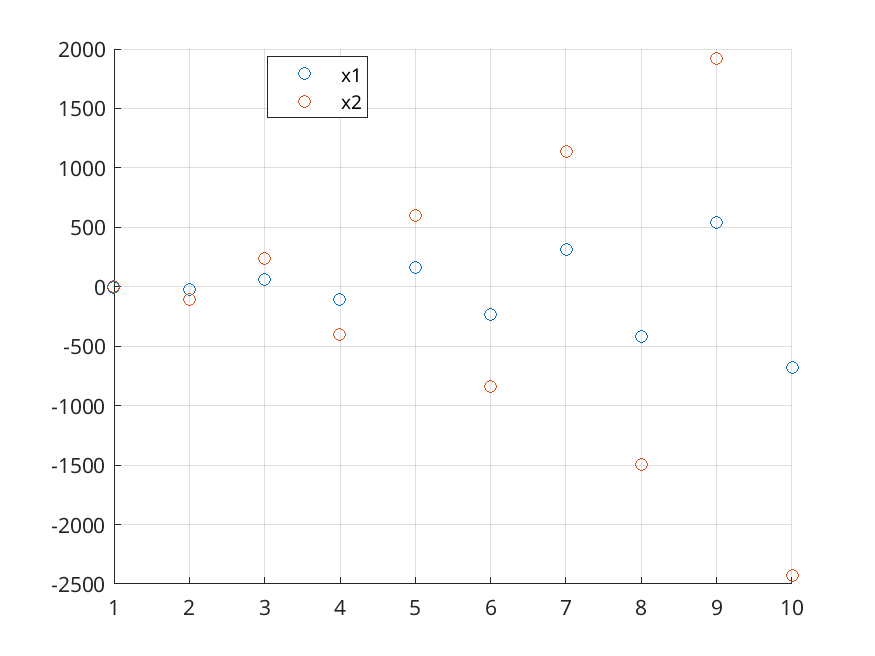
\includegraphics[scale=0.75]{./images/disk9.png}
		\caption{Графики $x_1$ и $x_2$ для начального условия $(-4, 1)$}
	\end{figure}
	
	\subsection{Собственные значения $\lambda_{1,2}=\pm id=\pm i \frac{9}{8}$}
	Матрица:
	$$
	A = \begin{bmatrix}
		0 & -\frac{9}{8} \\
		\frac{9}{8} & \phantom{-}0
	\end{bmatrix}
	$$
	
	\pagebreak
	Визуализация будет следующей:
	\begin{figure}[h]
		\centering
		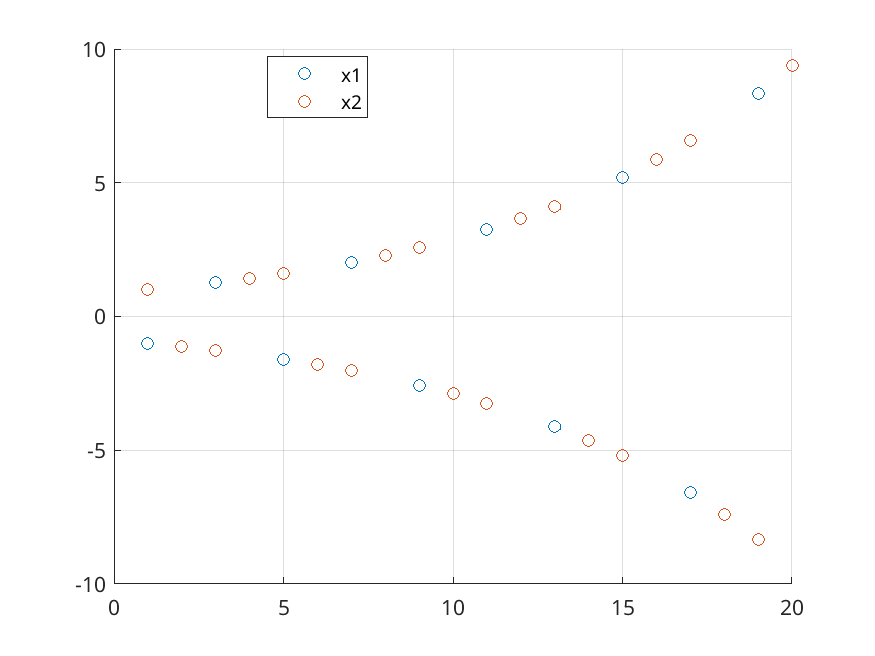
\includegraphics[scale=0.75]{./images/disk10.png}
		\caption{Графики $x_1$ и $x_2$ для начального условия $(-1, 1)$}
	\end{figure}
	
	\subsection{Собственные значения $\lambda_{1,2}=d=\frac{9}{8}$}
	
	Получим матрицу из сингулярного разложения
	$$
	A = \begin{bmatrix}
		10 & 12 \\
		16 & 14
	\end{bmatrix}
	\begin{bmatrix}
		\frac{9}{8} & 104 \\
		0 & \frac{9}{8}
	\end{bmatrix}
	\begin{bmatrix}
		10 & 12 \\
		16 & 14
	\end{bmatrix}^{-1}
	=
	\begin{bmatrix}
		\frac{2569}{8} & -200 \\ \\
		512 & -\frac{2551}{8}
	\end{bmatrix}
	$$
	
	\pagebreak
	Визуализация:
	\begin{figure}[h]
		\centering
		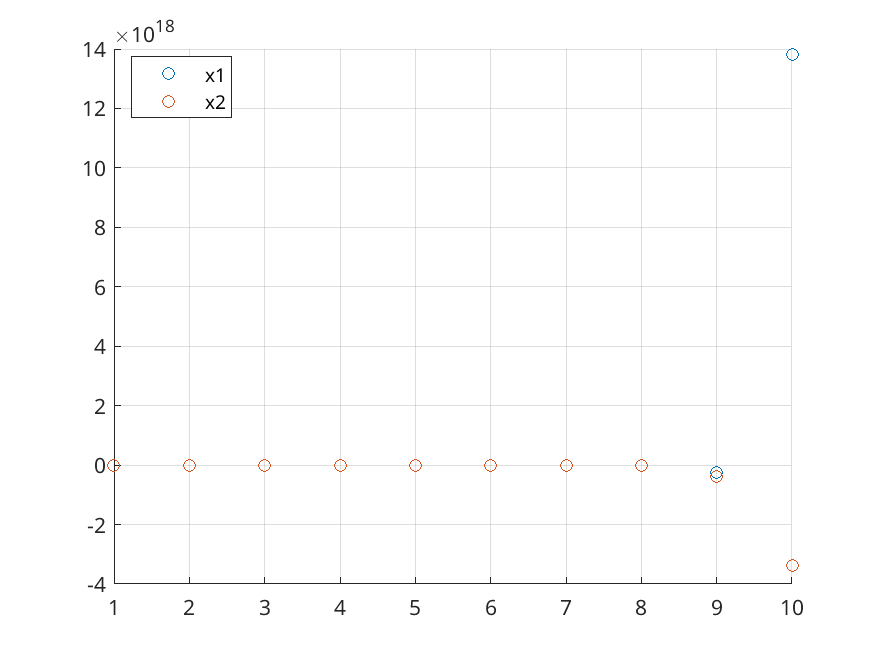
\includegraphics[scale=0.75]{./images/disk11.png}
		\caption{Графики $x_1$ и $x_2$ для начального условия $(0, 1)$}
	\end{figure}
	
	\subsection{Собственные значения $\lambda_{1,2}=0$}
	Матрица:
	$$
	A = \begin{bmatrix}
		3 & -1 \\
		9 & -3
	\end{bmatrix}
	$$
	
	\pagebreak
	Визуализация следующая:
	\begin{figure}[h]
		\centering
		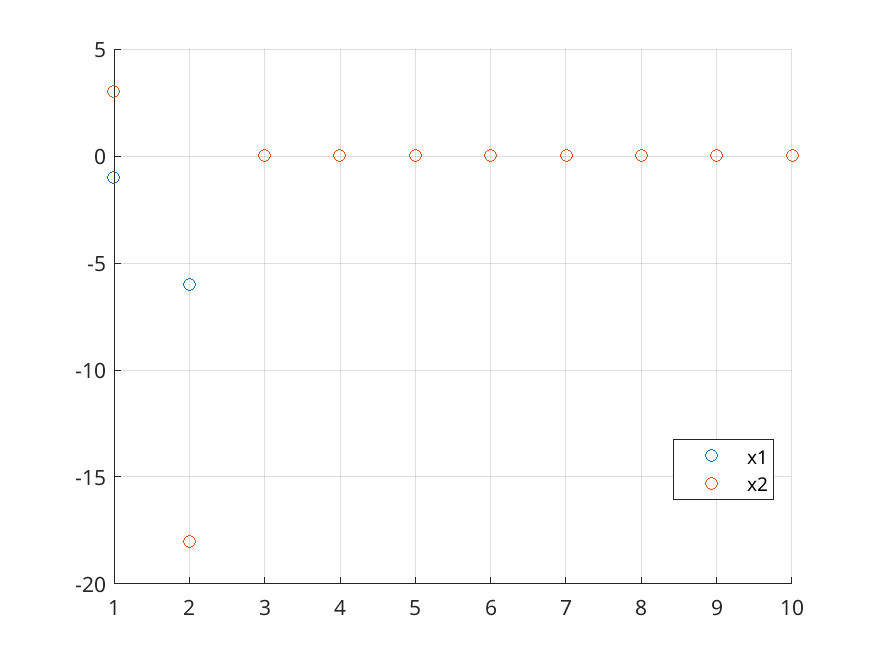
\includegraphics[scale=0.75]{./images/disk12.png}
		\caption{Графики $x_1$ и $x_2$ для начального условия $(-1, 3)$}
	\end{figure}
	
	\subsection*{Анализ влияния собственных значений}
	
	Из вышеприведенных графиков и ситуаций можно сделать вывод, что наша динамическая дискретная система является асимптотически устойчивой, если $|\lambda_i|<1$; неустойчивой - в случае $|\lambda_i|>1$ и является неким фокусом, то есть <<вертится>> около 0, при $|\lambda_i|=1$. То есть в дискретных системах на устойчивость влияет не только вещественная часть, но и комплексная, в чем мы неоднократно убеждались на примерах с чисто мнимыми собственными числами.
	
	Графически это можно представлять так: если мы попали внутрь круга радиуса 1, то мы наша система рано или поздно потухнет, уйдя в точку (0, 0); если на окружность того же радиуса, то будем <<крутиться>>, если же мы вышли за пределы нашего круга, то пиши пропал - ты улетишь в бесконечность с любыми ненулевыми начальными условиями...
	
	\section{Осцилятор?}
	
	Рассмотрим непрерывную систему вида 
	\begin{equation*}
		\begin{cases}
			\dot{x}_1 &= \, x_2\\
			\dot{x}_2 &=  a x_1 + b x_2
		\end{cases}\,.
	\end{equation*}
	
	И зададим её матрицей
	$$
	A = \begin{bmatrix}
		0 & 1 \\
		a & b
	\end{bmatrix}
	$$
	
	Проанализируем теперь устойчивость системы и характер её движения при различных значениях параметров $a$ и $b$.
	
	\subsection{$a<0, \text{ } b = 0$}
	Получаем следующее характеристическое уравнение:
	$$
	\lambda^2-a=0 \Rightarrow \lambda=\pm\sqrt{|a|}i \Rightarrow \text{Re}\lambda=0
	$$
	
	Вещественная часть равна 0, то система является статичной, то есть в виде интегральных кривых получаем эллипсы с центром в $(0, 0)$.
	
	\subsection{$a<0, \text{ } b < 0$}
	Характеристическое уравнение будет следующим:
	$$
	\lambda^2-\lambda b - a = 0
	$$
	
	Рассмотрим теперь различные ситуации:
	
	1. $b^2+4a <= 0$. Здесь устойчивость системы задаёт $\frac{b}{2}$, то есть если $b\in(-2, 0)$, то система является асимптотически устойчивой, если $b<-2$ - неустойчивой, и устойчивой в противном случае.
	
	2. $b^2+4a > 0$. Устойчивость в данном случае задаётся полным решением через дискриминант для $\lambda$.
	
	\subsection{$a>0, \text{ } b = 0$}
	Можем сразу получить наши собственные значения: $\lambda^2=a\Rightarrow\lambda=\pm\sqrt{a}$. При $a = 0$ получаем устойчивый узел, при остальных - устойчивый лишь в одном из направлений.
	
	\subsection{$a>0, \text{ } b < 0$}
	Этот случай по своей сути аналогичен пункту 2 (даже характеристическое уравнение то же), нужно лишь взять в качестве интервалов не отрицательные $b$, а положительные.
	
	\section{Физические системы}
	Кладезью для различные физических систем является второй закон Ньютона, используем его и для генерации физических систем.
	\subsection{Когда $b=0$}
	Пусть $x_1 = v$ - скорость материальной точки, $x_2 = \frac{F}{m}$, где $F$ - равнодействующая сил, m - масса, и пусть $F = \beta x$, тогда $\dot{x}_1=\frac{F}{m}=x_2$, а $\dot{x}_2=\frac{\beta}{m}v=\frac{\beta}{m}x_1$. Коэффициент $\beta$ здесь отвечает либо за постоянный разгон тела (представим, что мы стоим возле вентилятора), либо за замедление (здесь представим, что мы шагаем песку и с каждым метром становимся всё более и более медленными).
	\subsection{Общий случай}
	Случай, когда $b \neq 0$, ничем не сложнее, ведь нам всего лишь нужно добавить к нашей силе ещё одну составляющую: $F=\beta x + \alpha v$ (в данном случае коэффициент $\alpha$ отвечает либо за ускорение тела, либо за его замедление в зависимости от скорости). Нетрудно убедиться, что таким образом мы покроем все оставшиеся случаи.
	
	\textbf{На этом всё, спасибо!}
\end{document}
